\chapter{Empirical Evaluation}
\label{sec:eval}

We conducted an empirical evaluation on a set of 21 basic source code analyses
and 2 public massive code datasets to evaluate several factors about our hybrid
approach for selecting and optimizing traversal strategies.
First, we show the benefit of using our optimized selected traversal over
standard ones by evaluating the \emph{reduction in running times} of our hybrid
approach over the standards ones (\secref{sec:performance-gain}).
Then, we evaluate the correctness of the analysis results using our hybrid
approach to show that the decision analyses and optimizations in our approach
does not affect the correctness of the source code analyses
(\secref{sec:soundness}).
We also evaluate the precision of our selection algorithm by measuring how often
the hybrid approach selects the most time-efficient traversal
(\secref{sec:prediction-accuracy}).
Finally, we evaluate how the different components in the approach and different
kinds of static and runtime properties impact the overall performance? This is
done in \secref{sec:analysis-decision-tree} and
\secref{sec:analysis-traversal-opt}, and via various insight analysis of our
results.

%\noindent
%%
%\textbf{RQ1.} \emph{How much reduction in running time can be achieved using 
%our hybrid approach?} The answer to this shows the benefit of using our 
%optimized selected traversal over standard ones.
%
%\noindent
%%
%\textbf{RQ2.} \emph{Are the analysis results correct using the hybrid approach?}
 %This will show that the decision analyses and optimizations in our approach 
%does not affect the correctness of the source code analyses' results.
%
%\noindent
%%
%\textbf{RQ3.} \emph{How often does the hybrid approach select the most 
%time-efficient traversal?} 
%
%\noindent
%%
%\textbf{RQ4.} \emph{How do the different components in the approach and 
%different kinds of static and runtime properties impact the overall 
%performance?} This is done by various insight analysis of our evaluation 
%results.

\section{Analyses, Datasets and Experiment Setting}
\label{sec:exp-settings}

\begin{table*}[t]
	\scriptsize
  \centering
  \caption{List of source code analyses and the properties of their involved 
	traversals.}
	%\setlength{\tabcolsep}{5.5pt}
\begin{tabular}{rrrcccccrccc}
\toprule
      & \multicolumn{1}{c}{Analysis} & \multicolumn{1}{c}{Ts} & \multicolumn{3}{c}{$t_1$} & \multicolumn{3}{c}{$t_2$} & \multicolumn{3}{c}{$t_3$} \\
\cmidrule(lr){4-6} \cmidrule(lr){7-9} \cmidrule(lr){10-12}
      & \multicolumn{1}{c}{} & \multicolumn{1}{c}{} & Flw   & Lp  & Dir & Flw   & Lp  & \multicolumn{1}{c}{Dir} & Flw   & Lp  & Dir \\
\midrule
1     & Copy propagation (CP) & 3     & \xmark & \xmark & ---   & \cmark & \cmark & $\rightarrow$ & \xmark & \xmark & --- \\
2     & Common sub-expression detection (CSD) & 3     & \xmark & \xmark & ---   & \cmark & \cmark & $\rightarrow$ & \xmark & \xmark & --- \\
3     & Dead code (DC) & 3     & \xmark & \xmark & ---   & \cmark & \cmark & $\leftarrow$ & \xmark & \xmark & --- \\
4     & Loop invariant code (LIC) & 3     & \xmark & \xmark & ---   & \cmark & \cmark & $\rightarrow$ & \xmark & \xmark & --- \\
5    & Upsafety analysis (USA) & 3     & \xmark & \xmark & ---   & \cmark & \cmark & $\rightarrow$ & \xmark & \xmark & --- \\
6    & Valid FileReader (VFR) & 3     & \xmark & \xmark & ---   & \cmark & \cmark & $\rightarrow$ & \xmark & \xmark & --- \\
7    & Mismatched wait/notify (MWN) & 3     & \xmark & \xmark & ---   & \cmark & \cmark & $\rightarrow$ & \xmark & \xmark & --- \\
8     & Available expression (AE)  & 2     & \xmark & \xmark & ---   & \cmark & \cmark & $\rightarrow$ & \cellcolor{lightgray} & \cellcolor{lightgray} & \cellcolor{lightgray} \\
9     & Dominator (DOM)  & 2     & \xmark & \xmark & ---   & \cmark & \xmark & $\rightarrow$ & \cellcolor{lightgray} & \cellcolor{lightgray} & \cellcolor{lightgray} \\
10     & Local may alias (LMA) & 2     & \xmark & \xmark & ---   & \cmark & \cmark & $\rightarrow$ & \cellcolor{lightgray} & \cellcolor{lightgray} & \cellcolor{lightgray} \\
11     & Local must not alias (LMNA) & 2     & \xmark & \xmark & ---   & \cmark & \cmark & $\rightarrow$ & \cellcolor{lightgray} & \cellcolor{lightgray} & \cellcolor{lightgray} \\
12     & Live variable (LV) & 2     & \xmark & \xmark & ---   & \cmark & \cmark & $\leftarrow$ & \cellcolor{lightgray} & \cellcolor{lightgray} & \cellcolor{lightgray} \\
13    & Nullness analysis (NA) & 2     & \xmark & \xmark & ---   & \cmark & \cmark & $\rightarrow$ & \cellcolor{lightgray} & \cellcolor{lightgray} & \cellcolor{lightgray} \\
14    & Post dominator (PDOM) & 2     & \xmark & \xmark & ---   & \cmark & \xmark & $\leftarrow$ & \cellcolor{lightgray} & \cellcolor{lightgray} & \cellcolor{lightgray} \\
15    & Reaching definition (RD)  & 2     & \xmark & \xmark & ---   & \cmark & \cmark & $\rightarrow$ & \cellcolor{lightgray} & \cellcolor{lightgray} & \cellcolor{lightgray} \\
16    & Resource status (RS) & 2     & \xmark & \xmark & ---   & \cmark & \cmark & $\rightarrow$ & \cellcolor{lightgray} & \cellcolor{lightgray} & \cellcolor{lightgray} \\
17    & Very busy expression (VBE)  & 2     & \xmark & \xmark & ---   & \cmark & \cmark & $\leftarrow$ & \cellcolor{lightgray} & \cellcolor{lightgray} & \cellcolor{lightgray} \\
18    & Safe Synchronization (SS) & 2     & \xmark & \xmark & ---   & \cmark & \cmark & $\rightarrow$ & \cellcolor{lightgray} & \cellcolor{lightgray} & \cellcolor{lightgray} \\
19    & Used and defined variable (UDV) & 1     & \xmark & \xmark & ---   & \cellcolor{lightgray} & \cellcolor{lightgray} & \multicolumn{1}{c}{\cellcolor{lightgray}} & \cellcolor{lightgray} & \cellcolor{lightgray} & \cellcolor{lightgray} \\
20    & Useless increment in return (UIR) & 1     & \xmark & \xmark & ---   & \cellcolor{lightgray} & \cellcolor{lightgray} & \multicolumn{1}{c}{\cellcolor{lightgray}} & \cellcolor{lightgray} & \cellcolor{lightgray} & \cellcolor{lightgray} \\
21    & Wait not in loop (WNIL) & 1     & \xmark & \xmark & ---   & \cellcolor{lightgray} & \cellcolor{lightgray} & \multicolumn{1}{c}{\cellcolor{lightgray}} & \cellcolor{lightgray} & \cellcolor{lightgray} & \cellcolor{lightgray} \\
\bottomrule
\end{tabular}%
  \label{tab:analysis-table}%
\end{table*}%


\subsection{Analyses.} We collected source code analyses that traverse control flow 
graphs from textbooks and source code analysis tools. We also made sure that the 
analyses list covers all the static properties discussed in  
\secnref{sec:compute-properties}, i.e., data-flow sensitivity, loop sensitivity and 
traversal direction. We ended up with 21 source code analyses as shown in 
\tabref{tab:analysis-table}. They include 10 basic ones (analyses 1, 2, 8, 9, 
10, 11, 12, 14, 15 and 19) from textbooks (~\cite{compilers, programanalysis}) and 11 
tothers for detecting source code bugs, and code smells from the Soot 
framework (~\cite{vallee1999soot}) (analyses 3, 4, 5, 13, 17 and 18), and 
FindBugs tool (~\cite{findbugs-paste2007}) (analyses 6, 7, 16, 20 and 21). 
%We included analysis that needs control flow information to act upon. 
%The standard textbook analysis were chosen since these are the base analysis upon which more complicated analysis act on.
\tabref{tab:analysis-table} also shows the number of traversals each analysis 
contains and their static properties as described in \secref{sec:compute-properties}. 
%Most analyses have 2 traversals and all the first traversals are flow-insensitive and loop-insensitive.
The sets of traversals cover all types of static properties for 
flow-sensitivity, loop-sensitivity and direction (forward, backward and iterative).
All analyses are intra-procedural. We implemented all twenty one of these analysis using Boa language(~\cite{dyer2013boa}). The source code of these analyses are provided in the appendix. In \tabref{tab:analysis-table}, Ts denotes total number of traversals, $t_i$ denotes properties of traversal $i$-th, \emph{Flw} denotes data-flow sensitive, \emph{Lp} denotes loop sensitive,
\emph{Dir} denotes traversal direction where ---, $\rightarrow$ and $\leftarrow$ 
mean iterative, forward and backward, respectively.
%For expressing these analyses, we made use of Boa language~\cite{dyer2013boa}. Boa is a domain-specific language for mining open-source software repositories at the large scale. We extended Boa data schema to support the graph data structure and extended its syntax to support program analysis constructs described in~ \secref{sec:language}.

\begin{table*}[t]
\scriptsize
\centering
\caption{Statistics of the generated control flow graphs from two datasets.}
%\setlength{\tabcolsep}{5pt}
\begin{tabular}{lrrrrrr}
\toprule
\multicolumn{1}{c}{Dataset} & \multicolumn{1}{c}{All graphs} & \multicolumn{1}{c}{Sequential} & \multicolumn{1}{c}{Branches} & \multicolumn{3}{c}{Loops} \\
\cmidrule(lr){5-7}      &       &       &       & \multicolumn{1}{c}{All graphs} & \multicolumn{1}{c}{Branches} & \multicolumn{1}{c}{No branches} \\
\midrule
DaCapo & 287K & 186K (65\%) & 73K (25\%) & 28K (10\%) & 21K (7\%) & 7K (2\%)\\
GitHub & 161,523K & 111,583K (69\%) & 33,324K (21\%) & 16,617K (10\%) & 11,674K (7\%) & 4,943K (3\%) \\
\bottomrule
\end{tabular}%
\label{tab:dataset-table}%
\end{table*}%


\begin{table}
%\begin{table}[ht!]
	\centering
	\scriptsize
	\caption{Time contribution of each phase (in miliseconds).}
\setlength{\tabcolsep}{4.5pt}
\begin{tabular}{rrrrrrrr}
\toprule
Analysis & \multicolumn{2}{c}{Avg. Time} & Static & \multicolumn{4}{c}{Runtime} \\
\cmidrule(lr){2-3} \cmidrule(lr){5-8}      & DaCapo & GitHub &       & \multicolumn{2}{c}{DaCapo} & \multicolumn{2}{c}{GitHub} \\
\cmidrule(lr){5-6} \cmidrule(lr){7-8}      &       &       &       & Avg.  & Total & Avg.  & Total \\
\midrule
\multicolumn{1}{l}{CP} & 0.21 &    0.008   &       53  &   0.21    &  62,469     &    0.008   & 1359K \\
\multicolumn{1}{l}{CSD} & 0.19 &  0.012     &       60  &     0.19  &   56,840    &   0.012    &  1991K \\
\multicolumn{1}{l}{DC} & 0.19 &   0.010    &       45  &    0.19   &  54,822     &   0.010    &  1663K \\
\multicolumn{1}{l}{LIC} & 0.21 &  0.006     &       69  &    0.20   &    60,223   &    0.006   &  992K \\
\multicolumn{1}{l}{USA} & 0.19 &   0.006    &       90  &   0.19    &   54,268    &  0.009     &  1444K \\
\multicolumn{1}{l}{VFR} & 0.18 &    0.007   &       42  &   0.18    &     52,483  &   0.007    &  1142K \\
\multicolumn{1}{l}{MWN} & 0.18 &    0.006   &       36  &   0.18    &     52,165  &   0.006    &  1109K \\
\multicolumn{1}{l}{AE} & 0.18 &    0.007   &       43  &   0.18    &     53,290  &   0.007    &  1169K \\
\multicolumn{1}{l}{DOM} & 0.21 &    0.008   &       35  &    0.21   &    62,416    &  0.008     &  1307K \\
\multicolumn{1}{l}{LMA} & 0.18 &    0.008   &       76  &   0.18    &     52,483  &   0.008    &  1346K \\
\multicolumn{1}{l}{LMNA} & 0.18 &    0.008   &       80  &     0.18  &   53,182    &  0.008     &  1407K\\
\multicolumn{1}{l}{LV} & 0.17 &   0.007    &       32  &    0.17   &     49,231  &   0.007    &  1273K\\
\multicolumn{1}{l}{NA} & 0.16 &   0.008    &       64  & 0.16      &    46,589   &   0.008    &  1398K\\
\multicolumn{1}{l}{PDOM} & 0.20 &    0.012   &       34  &   0.20    &   57,203    &   0.012    &  2040K\\
\multicolumn{1}{l}{RD} & 0.20 &   0.007    &       48  &    0.20   &   57,359    &  0.007     &  1155K\\
\multicolumn{1}{l}{RS} & 0.16 &   0.006    &       28  &   0.16    &   46,367    &   0.006    &  996K\\
\multicolumn{1}{l}{VBE} & 0.17 &  0.006     &       44  &   0.17    &   49,138    &   0.006    &  1062K\\
\multicolumn{1}{l}{SS} & 0.17 &  0.006     &       32  &   0.17    &   48,990    &   0.006    &  1009K\\
\multicolumn{1}{l}{UDV} & 0.14 &  0.005     &       10  &    0.14   &  41,617     &  0.005     &  928K\\
\multicolumn{1}{l}{UIR} & 0.14 &   0.006    &       14  &   0.14    &   41,146    &   0.006    &  1020K\\
\multicolumn{1}{l}{WNIL} & 0.14 &   0.007    &       15  &   0.14    &  41,808     &  0.007     &  1210K\\
\bottomrule
\end{tabular}%

	\label{tab:time}%
%\end{table}
\end{table}%

%\begin{table}[t]
	%\centering
	%\scriptsize
	%\caption{Time contribution of each phase (in miliseconds).}
	%%\setlength{\tabcolsep}{5pt}
%% Table generated by Excel2LaTeX from sheet 'Sheet1'
%\begin{tabular}{rrccrrr}
%\toprule
%\multicolumn{1}{c}{Analysis} & \multicolumn{1}{c}{Static} & \multicolumn{4}{c}{DaCapo}            & \multicolumn{1}{c}{SourceForge} \\
%\cmidrule(lr){3-6} \cmidrule(lr){7-7}
%\multicolumn{1}{c}{} & \multicolumn{1}{c}{} & \multicolumn{2}{c}{CFG creation} & \multicolumn{2}{c}{Traversal} & \multicolumn{1}{c}{Traversal} \\
%\cmidrule(lr){3-4} \cmidrule(lr){5-6} \cmidrule(lr){7-7}
%\multicolumn{1}{c}{} & \multicolumn{1}{c}{} & Avg.  & Total & \multicolumn{1}{c}{Avg.} & \multicolumn{1}{c}{Total} & \multicolumn{1}{r}{Total} \\
%\midrule
%\multicolumn{1}{l}{CP} &          53  & \multirow{18}{*}{0.05} & \multirow{18}{*}{13,171} &    0.17  &          49,298  &      1,359K  \\
%\multicolumn{1}{l}{CSD} &          60  &       &       &    0.15  &          43,671  &      1,991K  \\
%\multicolumn{1}{l}{DC} &          45  &       &       &    0.15  &          41,651  &      1,663K  \\
%\multicolumn{1}{l}{LIC} &          69  &       &       &    0.16  &          47,123  &     1,092K  \\
%\multicolumn{1}{l}{USA} &          90  &       &       &    0.14  &          41,168  &      1,444K  \\
%\multicolumn{1}{l}{AE} &          43  &       &       &    0.14  &          40,190  &      1,169K  \\
%\multicolumn{1}{l}{DOM} &          35  &       &       &    0.17  &          49,316   &      1,307K  \\
%\multicolumn{1}{l}{LMA} &          76  &       &       &    0.14  &          39,383  &      1,346K  \\
%\multicolumn{1}{l}{LMNA} &          80  &       &       &    0.14  &          40,082  &     1,407K  \\
%\multicolumn{1}{l}{LV} &          32  &       &       &    0.13  &          36,131  &      1,273K  \\
%\multicolumn{1}{l}{NA} &          64  &       &       &    0.12  &          33,489  &      1,398K  \\
%\multicolumn{1}{l}{PDOM} &          34  &       &       &    0.15  &          44,103  &      2,040K  \\
%\multicolumn{1}{l}{RD} &          48  &       &       &    0.15  &          44,259  &      1,155K  \\
%\multicolumn{1}{l}{RS} &          28  &       &       &    0.12  &          33,267  &      996K  \\
%\multicolumn{1}{l}{VBE} &          44  &       &       &    0.13  &          36,038  &     1,062K  \\
%\multicolumn{1}{l}{UDV} &          10  &       &       &    0.10  &          28,517  &      928K  \\
%\multicolumn{1}{l}{UIR} &          14  &       &       &    0.10  &          28,046  &     1,020K  \\
%\multicolumn{1}{l}{WNIL} &          15  &       &       &    0.10  &          28,708  &      1,210K  \\
%\bottomrule
%\end{tabular}%
%
	%\label{tab:time-break-down-table}%
%\end{table}%

%\begin{table}[t]
	%\centering
	%\scriptsize
	%\caption{Time contribution of each phase (in miliseconds).}
	%\setlength{\tabcolsep}{5pt}
%\begin{tabular}{rrccrr}
%\toprule
%\multicolumn{1}{l}{Analysis} & Static & \multicolumn{2}{c}{CFG creation} & \multicolumn{2}{c}{Traversal} \\
%\cmidrule(lr){3-4} \cmidrule(lr){5-6}
%\multicolumn{1}{c}{} & \multicolumn{1}{c}{} & Avg.  & Total & \multicolumn{1}{c}{Avg.} & \multicolumn{1}{c}{Total} \\
%\midrule
%\multicolumn{1}{l}{CP} &         53  & \multirow{18}{*}{0.05} & \multirow{18}{*}{13,170} &           0.17  &    49,297  \\
%\multicolumn{1}{l}{CSD} &         60  &       &       &           0.15  &    43,670  \\
%\multicolumn{1}{l}{DC} &         45  &       &       &           0.15  &    41,651  \\
%\multicolumn{1}{l}{LIC} &         69  &       &       &           0.16  &    47,122  \\
%\multicolumn{1}{l}{USA} &         90  &       &       &           0.14  &    41,168  \\
%\multicolumn{1}{l}{AE} &         43  &       &       &           0.14  &    40,190  \\
%\multicolumn{1}{l}{DOM} &         35  &       &       &           0.17  &    49,316  \\
%\multicolumn{1}{l}{LMA} &         76  &       &       &           0.14  &    39,382 \\
%\multicolumn{1}{l}{LMNA} &         80  &       &       &           0.14  &    40,081  \\
%\multicolumn{1}{l}{LV} &         32  &       &       &           0.13  &    36,130  \\
%\multicolumn{1}{l}{NA} &         64  &       &       &           0.12  &    33,488  \\
%\multicolumn{1}{l}{PDOM} &         34  &       &       &           0.15  &    44,103  \\
%\multicolumn{1}{l}{RD} &         48  &       &       &           0.15  &    44,259  \\
%\multicolumn{1}{l}{RS} &         28  &       &       &           0.12  &    33,267  \\
%\multicolumn{1}{l}{VBE} &         44  &       &       &           0.13  &    36,037  \\
%\multicolumn{1}{l}{UDV} &         10  &       &       &           0.10  &    28,517  \\
%\multicolumn{1}{l}{UIR} &         14  &       &       &           0.10  &    28,046  \\
%\multicolumn{1}{l}{WNIL} &         15  &       &       &           0.10  &    28,708  \\
%\bottomrule
%\end{tabular}%
	%\label{tab:time-break-down-table}%
%\end{table}%


\subsection{Datasets.} We ran the analyses on two datasets: DaCapo 9.12 benchmark (~\cite{blackburn2006dacapo}), 
DaCapo for short, and a ultra-large-scale dataset containing projects from
GitHub from Boa.
%
DaCapo dataset contains the source code of 10 open source Java projects: 
Apache Batik, Apache FOP, Apache Aurora, Apache Tomcat, Jython, Xalan-Java, 
PMD, H2 database, Sunflow and Daytrader. GitHub dataset contains the 
source code of more than 380K Java projects collected from 
GitHub.com. Each method in the datasets was used to generate a control 
flow graph (CFG) on which the analyses would be run. The statistics of the 
two datasets are shown in \tabref{tab:dataset-table}. DaCapo dataset contains 
287K non-empty CFGs while GitHub dataset contains more than 162M. Both 
have similar distributions of CFGs over graph \graphprop{}. Most CFGs are sequential 
and only 10\% have loops.

\subsection{Setting.} We compared our \textit{hybrid} approach against the six 
standard traversal strategies in \secref{sec:candidates}: DFS, PO, RPO, WPO, 
WRPO and ANY. The running time for each analysis is measured from the start 
to the end of the analysis which includes constructing CFGs and traversing 
CFGs. The running time for our hybrid approach also includes the time for 
computing the static and runtime properties, making the traversal strategy 
decision, optimizing it and then using the optimized traversal strategy to 
traverse the CFG and run the analysis.
%
The analyses on DaCapo dataset were run on  a single machine with 24 GB of 
memory and 24-cores, running on Linux 3.5.6-1.fc17 kernel. Running analyses 
on GitHub dataset on a single machine would take weeks to finish, so analyses were executed on a Hadoop [Apache Software Foundation 2015a] install with 1 name node, 1 job tracker node, and 10 compute nodes. The compute nodes have a total of 148 CPU cores and 2GB memory per core. All machines run Ubuntu 12.04LTS. The cluster has been tuned for performance,including setting the maximum number of map tasks for each compute node equal to the number of cores on that node, increasing the VM heap size to 1GB per task, and enabling short-circuit local reads in the distributed filesystem.

%Our experiments were run on two modes.
%\begin{itemize}
%\item Sequential mode : Run on a single machine with 24 GB of memory and 24-cores, running
%on Linux 3.5.6-1.fc17 kernel.
%\item Cluster Mode : Programs  were  executed  on  a  standard  Hadoop 1.0.3
%install with 1 name node, 1 job tracker node, and 6 compute nodes.
%\end{itemize}

\chapter{Running Time and Time Reduction}
\label{sec:performance-gain}

We first report the running times and then study the achieved reductions against standard traversal strategies. 

\section{Running Time}

\tabref{tab:time} shows the running times for 21 analyses on the two 
datasets. On average (column \textbf{Avg. Time}), each analysis took 
0.14--0.21 ms and 0.005--0.012 ms to analyze a graph in Dacapo and GitHub 
datasets, respectively. The variation in the average analysis time is 
mainly due to the difference in the machines used to run the analysis for 
DaCapo and GitHub datasets, as described in Chapter 4.1. Also, the average 
sizes of graphs in DaCapo are much larger than the average sizes of the graphs in the GitHub.
%
Columns \textbf{Static} and \textbf{Runtime} show the time contributions for 
different components of the hybrid approach: the time for determining the 
static properties of each analysis which is done once for each analysis, and 
the time for constructing the CFG of each method and traversing the CFG which 
is done once for every constructed CFG. 
%From the results shown in table \ref{tab:time}, it can be seen that, about 70\%--80\% of the time 
%is contributed by the actual traversal and 20\%--25\% of the time is 
%contributed by CFG creation phase which also includes affixing dynamic 
%properties. 
We can see that the time for collecting static information is negligible, 
less than 0.2\% for DaCapo dataset and less than 0.01\% for GitHub 
dataset, when compared to the total runtime information collection time, as it is performed only 
once per traversal. When compared to the average runtime information collection time, the static 
time is quite significant. However, the overhead introduced by static 
information collection phase diminishes as the number of CFGs increases and 
becomes insignificant when running on those two large datasets. This result 
shows the benefit of our hybrid approach when applying on ultra-large-scale
analysis.

\section{Time Reduction}

%\begin{figure*}[ht!]
%\centering
%\textbf{a) \textit{DaCapo}}\\
%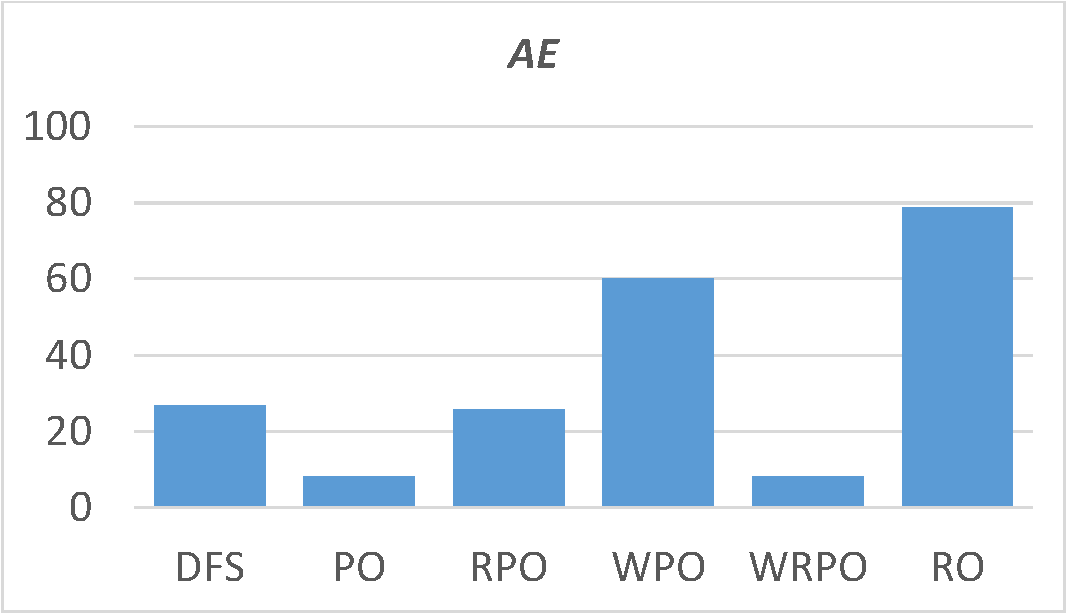
\includegraphics[width=0.32\linewidth]{ecoop-figures/ae-crop.pdf}
%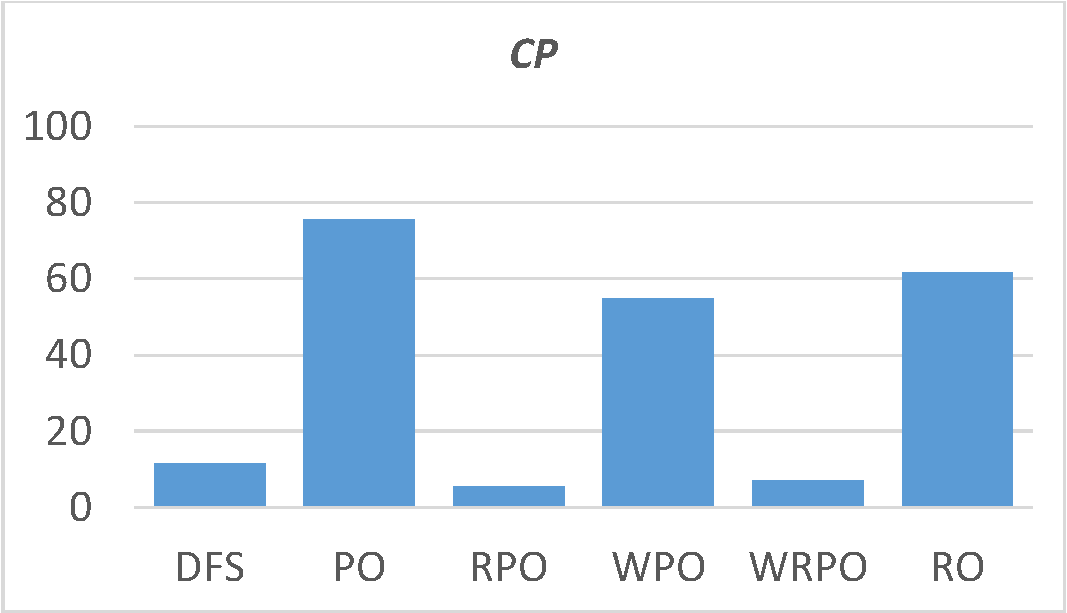
\includegraphics[width=0.32\linewidth]{ecoop-figures/cp-crop.pdf}
%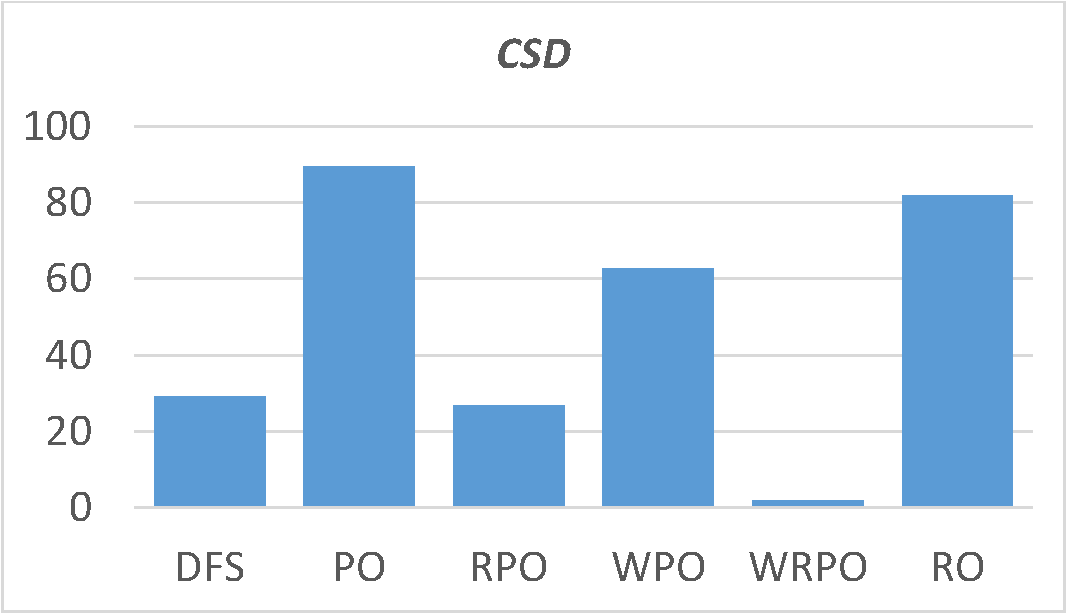
\includegraphics[width=0.32\linewidth]{ecoop-figures/csd-crop.pdf}
%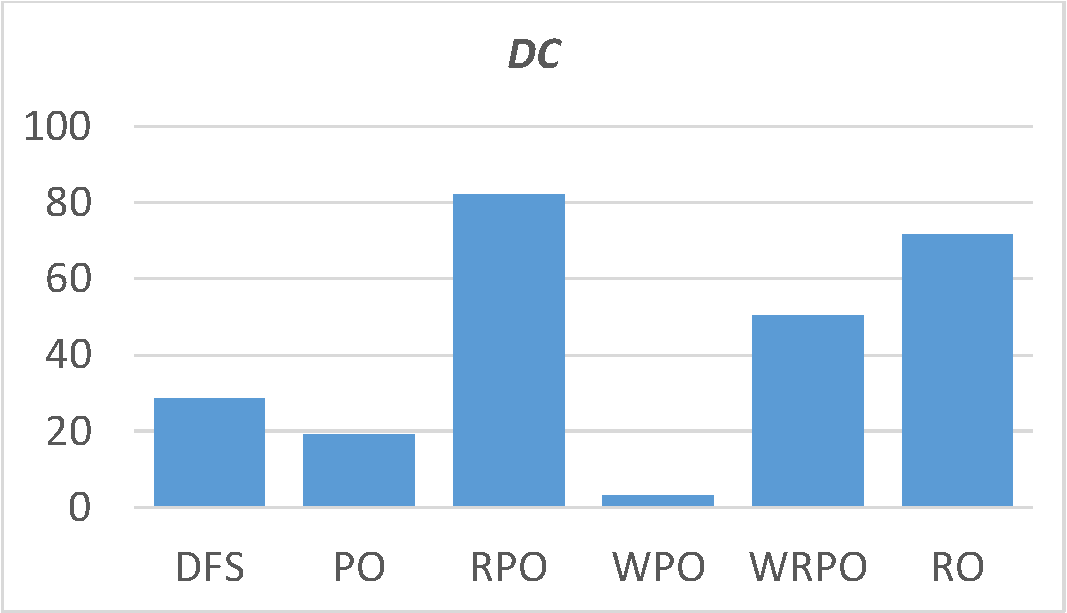
\includegraphics[width=0.32\linewidth]{ecoop-figures/dc-crop.pdf}
%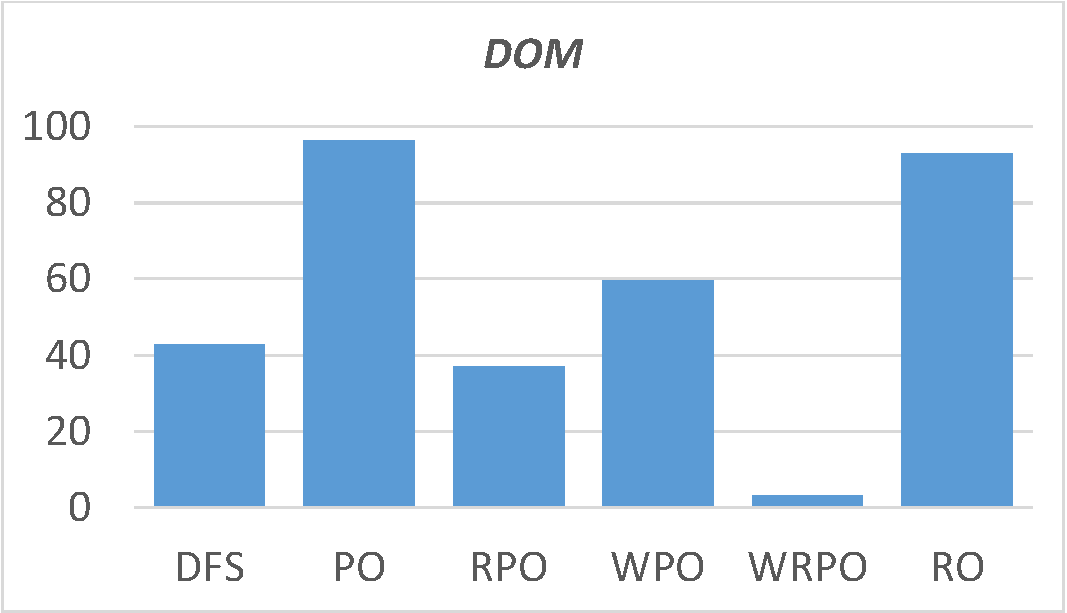
\includegraphics[width=0.32\linewidth]{ecoop-figures/dom-crop.pdf}
%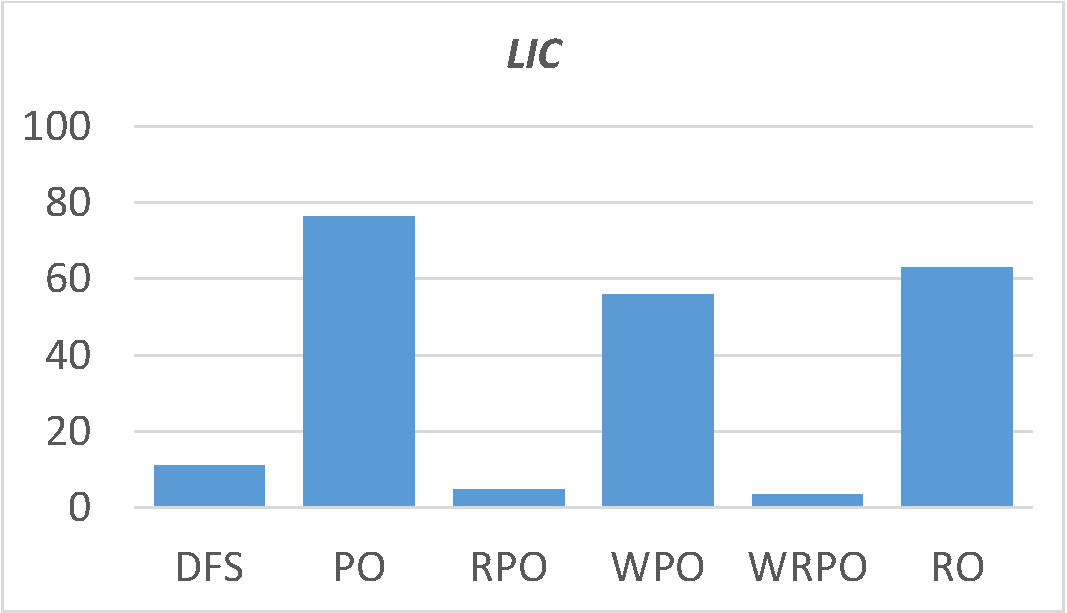
\includegraphics[width=0.32\linewidth]{ecoop-figures/lic-crop.pdf}
%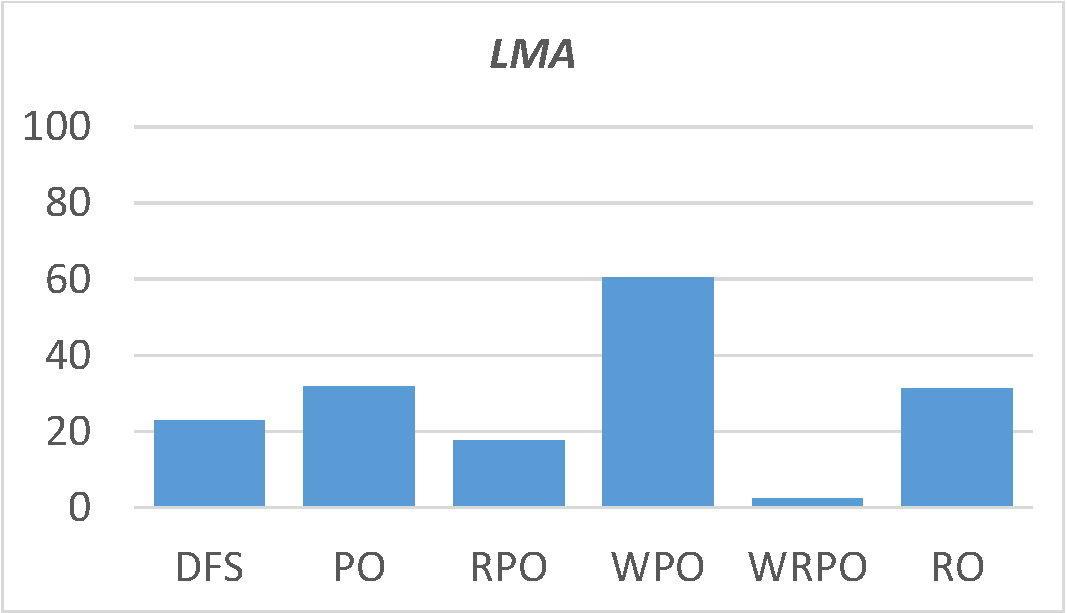
\includegraphics[width=0.32\linewidth]{ecoop-figures/lma-crop.pdf}
%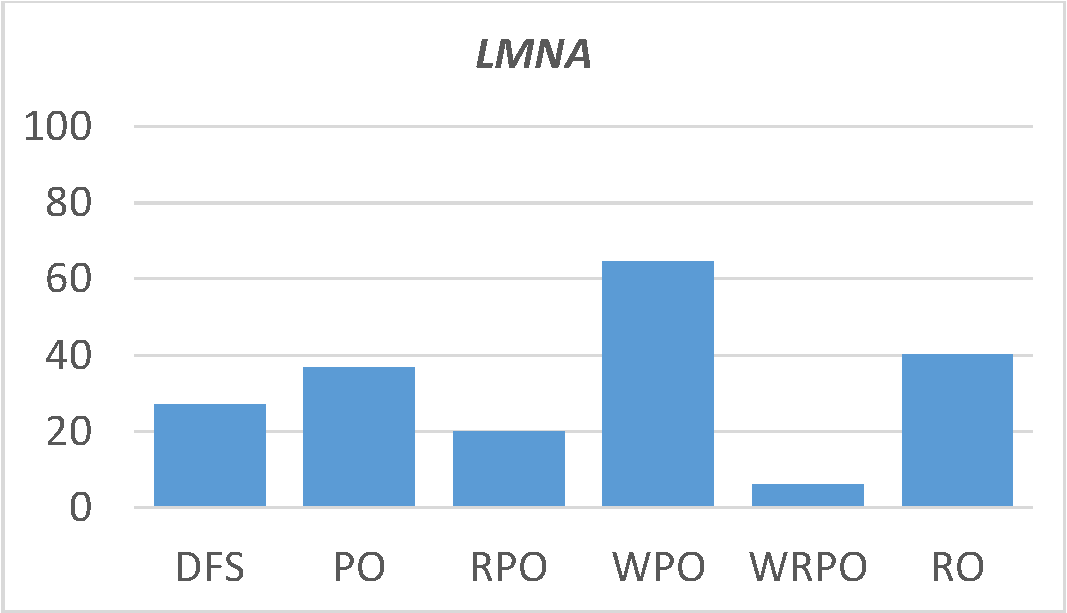
\includegraphics[width=0.32\linewidth]{ecoop-figures/lmna-crop.pdf}
%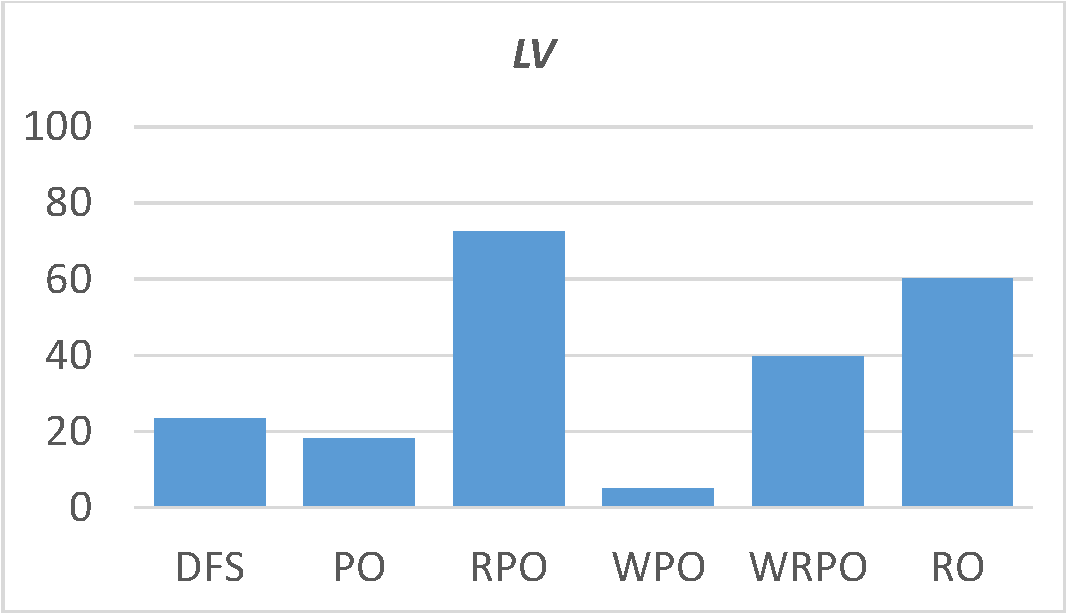
\includegraphics[width=0.32\linewidth]{ecoop-figures/lv-crop.pdf}
%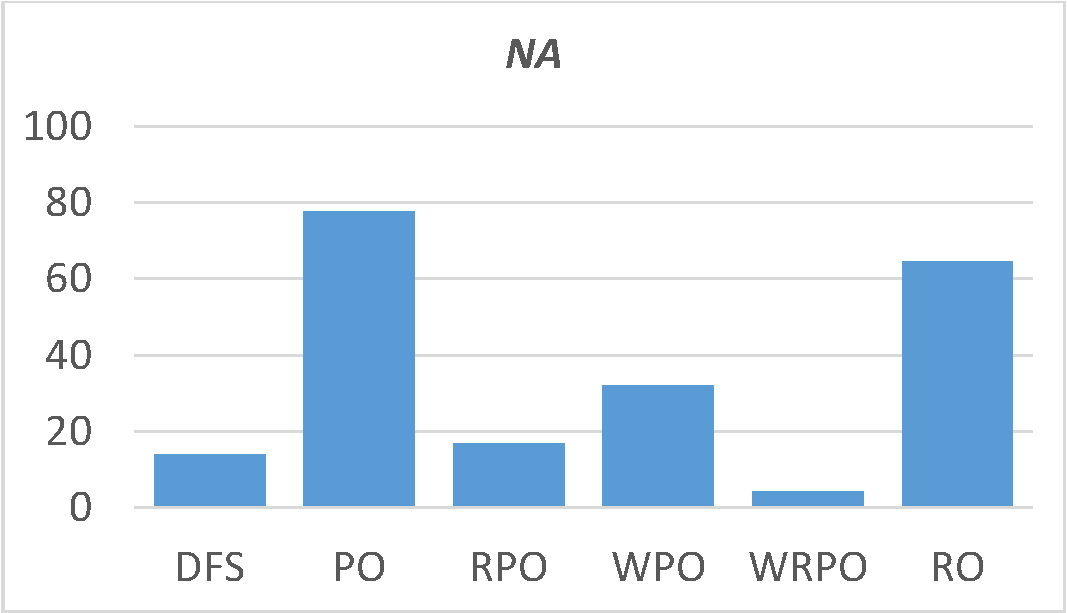
\includegraphics[width=0.32\linewidth]{ecoop-figures/na-crop.pdf}
%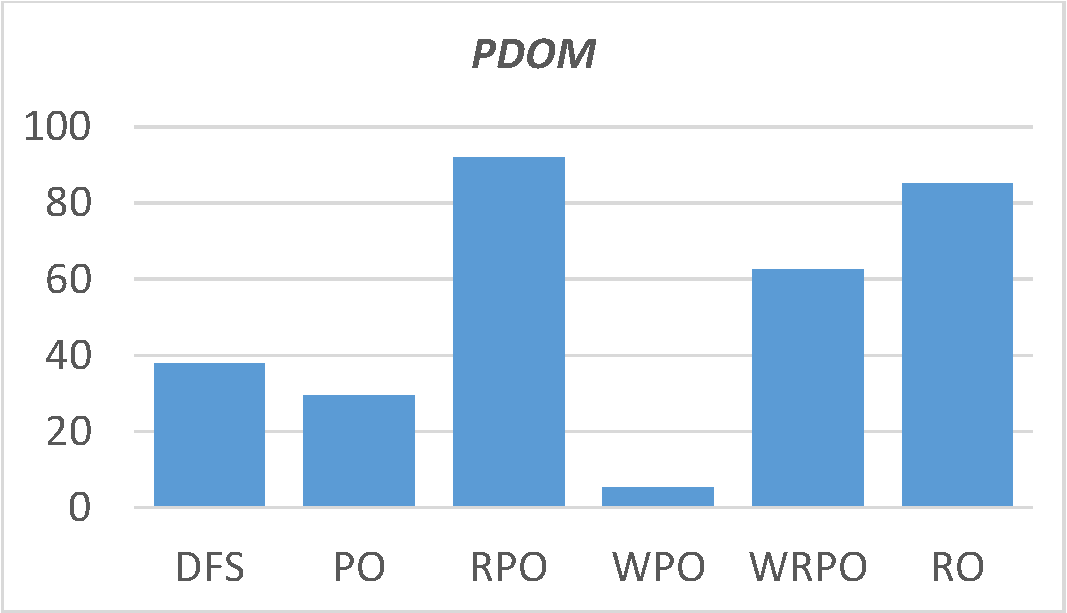
\includegraphics[width=0.32\linewidth]{ecoop-figures/pdom-crop.pdf}
%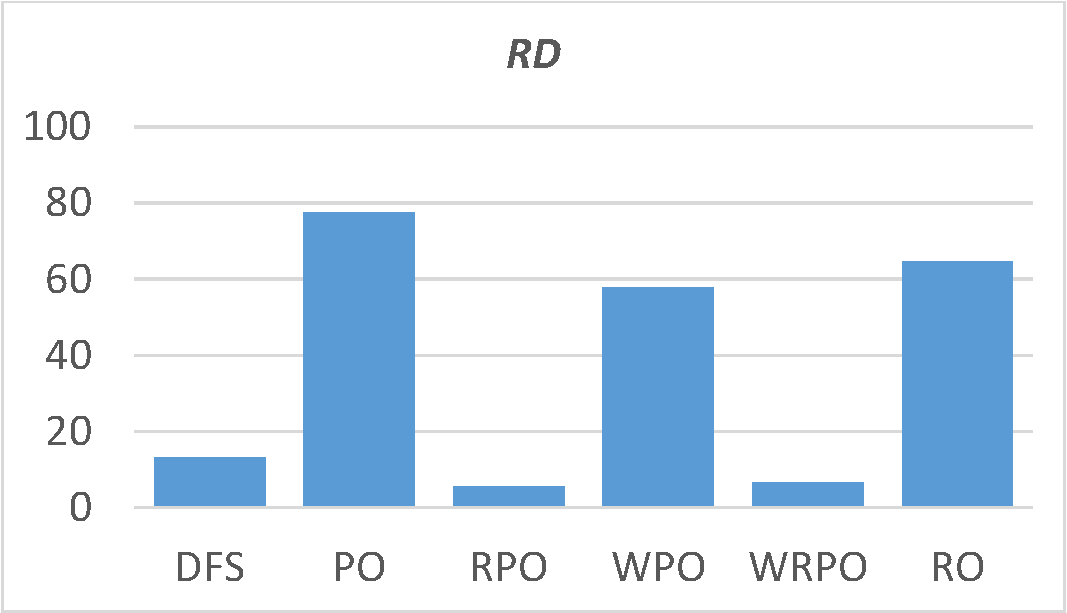
\includegraphics[width=0.32\linewidth]{ecoop-figures/rd-crop.pdf}
%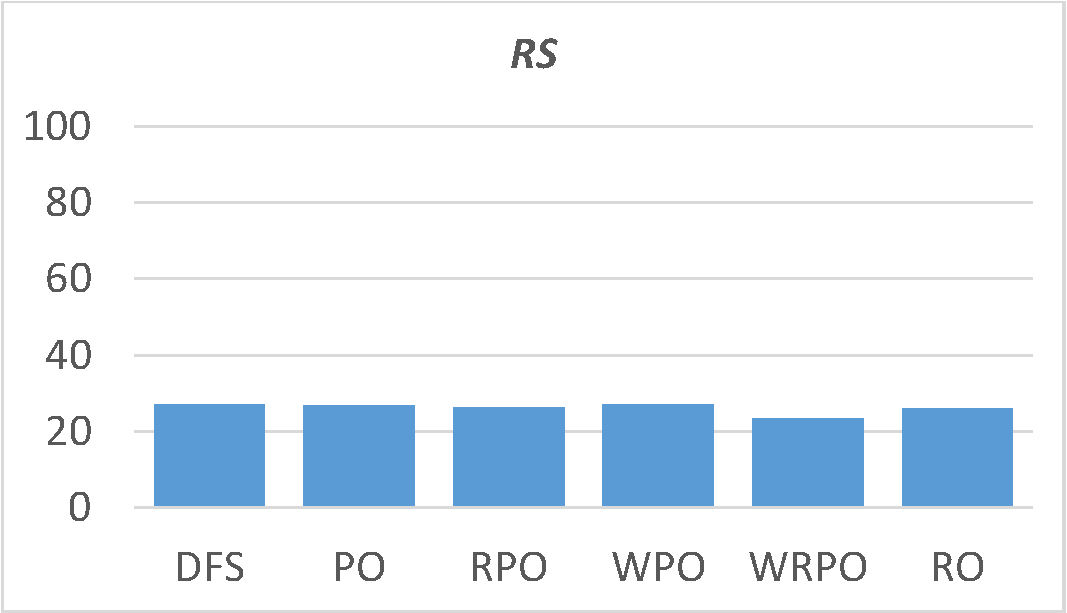
\includegraphics[width=0.32\linewidth]{ecoop-figures/rs-crop.pdf}
%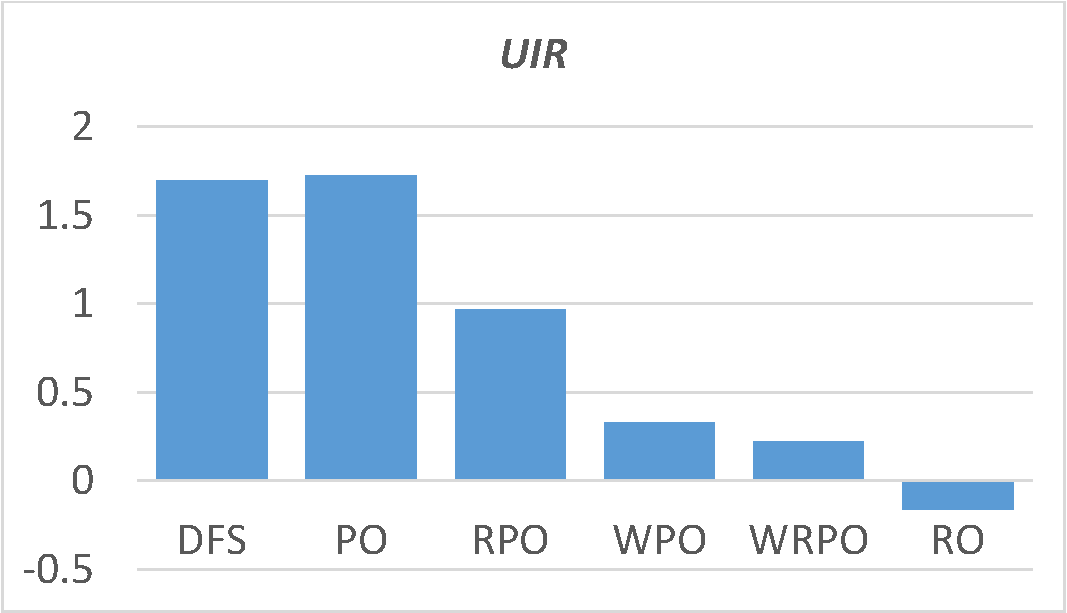
\includegraphics[width=0.32\linewidth]{ecoop-figures/uir-crop.pdf}
%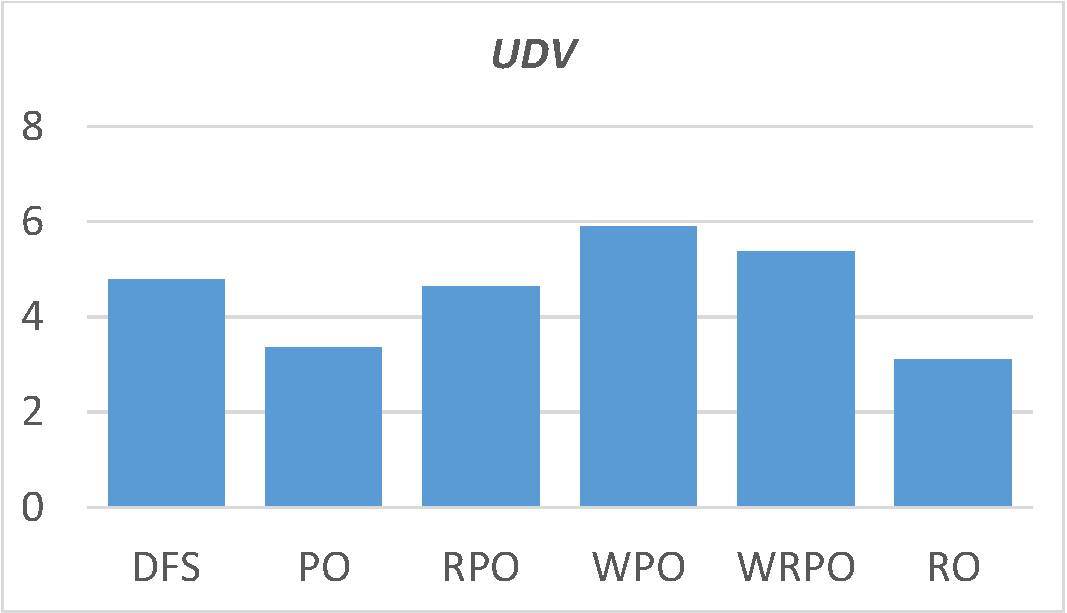
\includegraphics[width=0.32\linewidth]{ecoop-figures/udv-crop.pdf}
%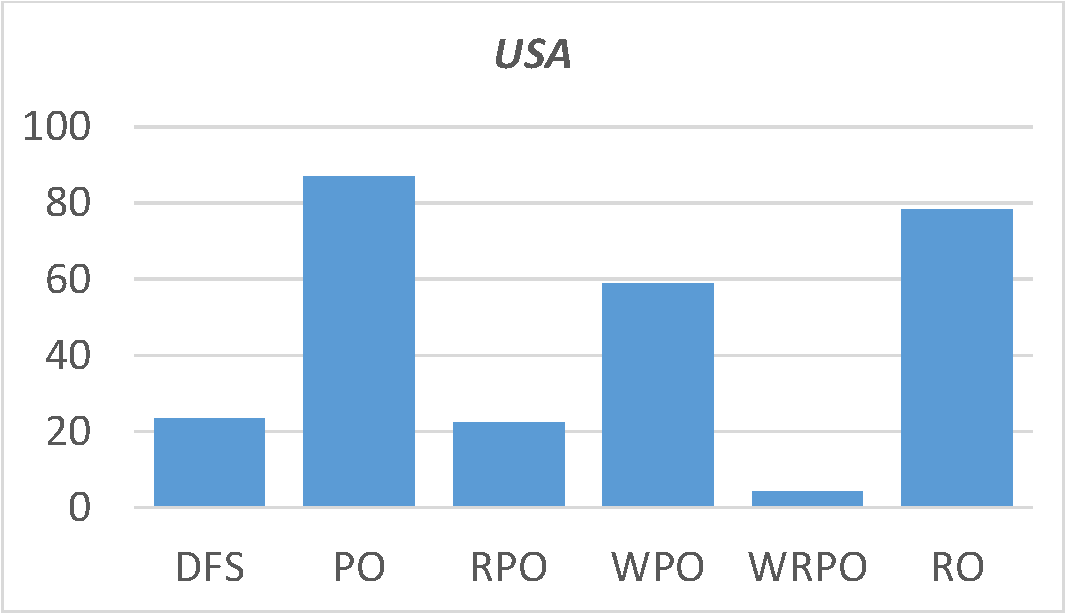
\includegraphics[width=0.32\linewidth]{ecoop-figures/usa-crop.pdf}
%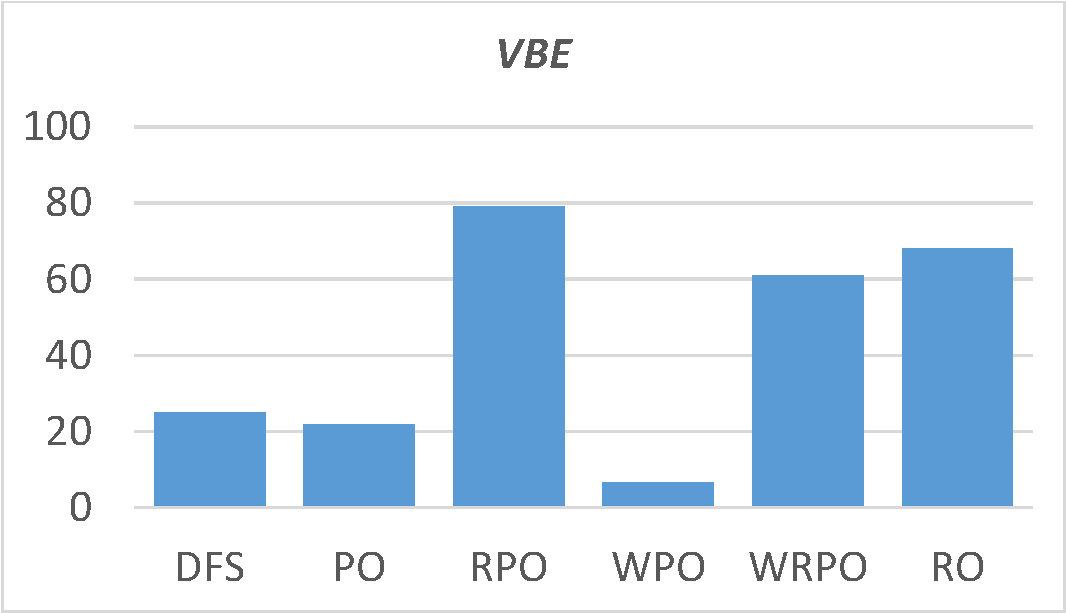
\includegraphics[width=0.32\linewidth]{ecoop-figures/vbe-crop.pdf}
%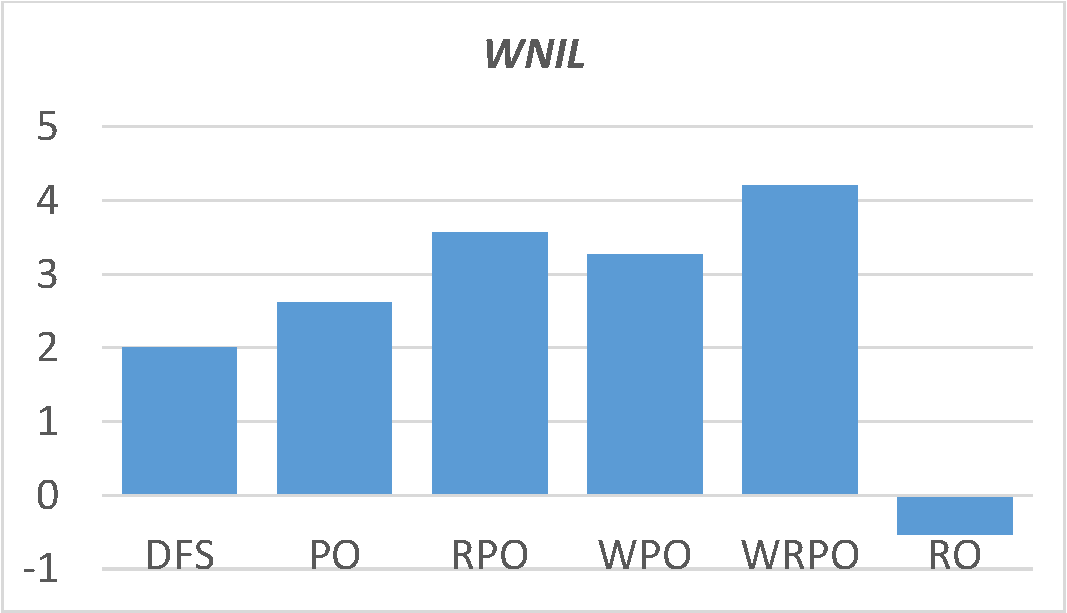
\includegraphics[width=0.32\linewidth]{ecoop-figures/wnil-crop.pdf}\newline
%\textbf{c) \textit{Overall}}\\
%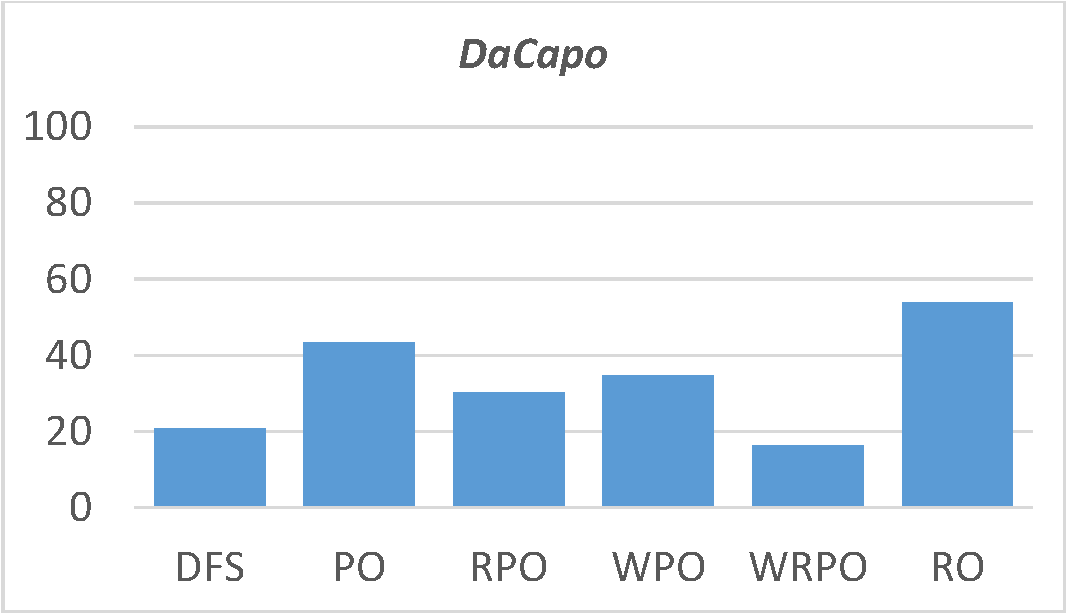
\includegraphics[width=0.32\linewidth]{ecoop-figures/dacapo-overall-crop.pdf}
  %\caption[Percentage reduction in execution time of hybrid approach over other candidate traversals on \textit{DaCapo} (Sequential mode) and \textit{SourceForge} (Cluster mode).]
%{Percentage reduction in execution time of hybrid approach over other candidate traversals on \textit{DaCapo} (Sequential mode) and \textit{SourceForge} (Cluster mode).
%\label{fig:dacapo-singlemachine-time-percentage}}
%\end{figure*}

%\begin{figure*}[ht!]
%\centering
%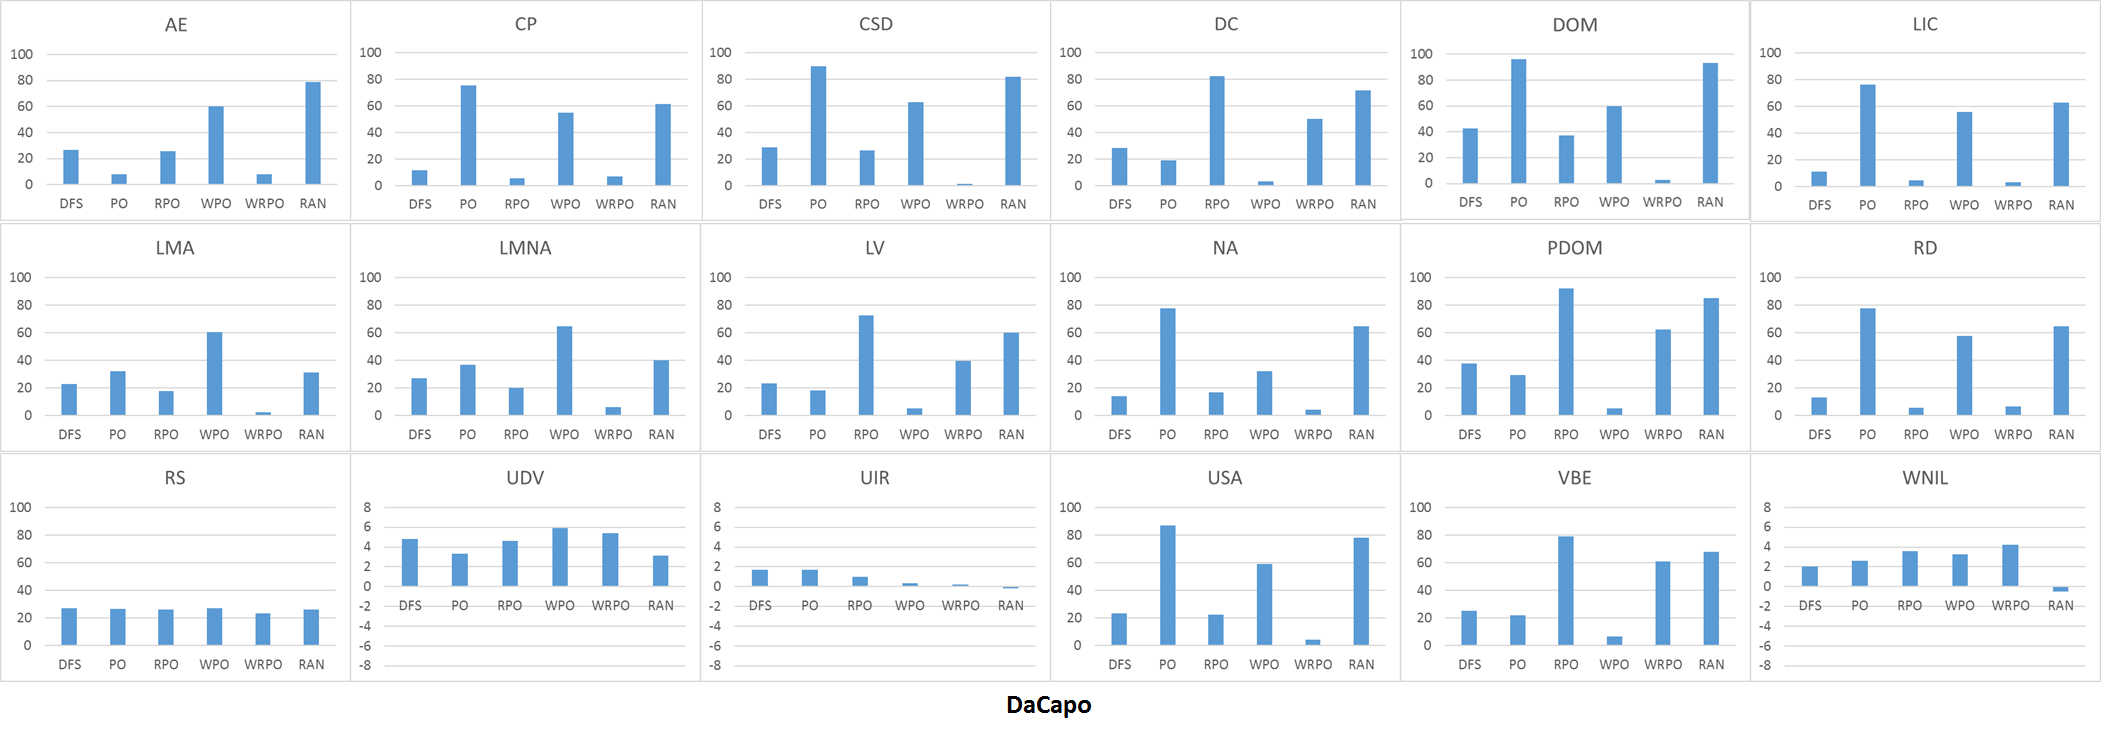
\includegraphics[width=\textwidth]{ecoop-figures/dacapo-seq-reduction.png}
%  \caption[Percentage reduction in execution time of hybrid approach over other candidate traversals on \textit{DaCapo} (Sequential mode), \textit{DaCapo} (Cluster mode), \textit{SourceForge} (Cluster mode).]
%{Percentage reduction in execution time of hybrid approach over other candidate traversals on \textit{DaCapo} (Sequential mode), \textit{DaCapo} (Cluster mode), \textit{SourceForge} (Cluster mode).
%\label{fig:dacapo-singlemachine-time-percentage}}
%\end{figure*}

\begin{figure*}[t]%
\centering
\scriptsize
\subfloat[Time reduction for each analysis.] {
\begin{tabular}{lrrrrrr|rrrrrr}
\toprule
\multicolumn{1}{l}{Analysis} & \multicolumn{6}{c|}{DaCapo}                    & \multicolumn{6}{c}{GitHub} \\
\cmidrule(lr){2-7} \cmidrule(lr){8-13}
      & DFS   & PO    & RPO   & WPO   & WRPO  & ANY    & DFS   & PO    & RPO   & WPO   & WRPO  & ANY \\
\midrule
\multicolumn{1}{l}{CP} & \cellcolor{lightblack}17\%  & \cellcolor{lightgreen}83\%  &  \cellcolor{lightblue}9\%   & \cellcolor{lightgreen}66\%  &  \cellcolor{lightblack}11\%   & \cellcolor{lightgreen}72\%  & \cellcolor{lightblack}17\%  & \cellcolor{lightgreen}88\%  &  \cellcolor{lightblack}12\%   & \cellcolor{lightgreen}80\%  &  \cellcolor{lightblue}5\%   & \cellcolor{lightgreen}82\% \\
\multicolumn{1}{l}{CSD} & \cellcolor{lightblack}41\%  & \cellcolor{lightgreen}93\%  & \cellcolor{lightblack}39\%  & \cellcolor{lightgreen}74\%  &  \cellcolor{lightblue}4\%   & \cellcolor{lightgreen}89\%  & \cellcolor{lightblack}31\%  & --  & \cellcolor{lightblack}24\%  & --  &  \cellcolor{lightblack}12\%   & -- \\
\multicolumn{1}{l}{DC} & \cellcolor{lightblack}41\%  & \cellcolor{lightblack}30\%  & \cellcolor{lightgreen}89\%  &  \cellcolor{lightblue}7\%   & \cellcolor{lightgreen}64\%  & \cellcolor{lightgreen}81\%  & \cellcolor{lightblack}25\%  & \cellcolor{lightblack}22\%  & --  &  \cellcolor{lightblue}7\%   & --  & -- \\
\multicolumn{1}{l}{LIC} & \cellcolor{lightblack}17\%  & \cellcolor{lightgreen}84\%  &  \cellcolor{lightblue}8\%   & \cellcolor{lightgreen}67\%  &  \cellcolor{lightblue}7\%   & \cellcolor{lightgreen}73\%  & \cellcolor{lightblack}19\%  & \cellcolor{lightgreen}89\%  &  \cellcolor{lightblack}15\%   & \cellcolor{lightgreen}81\%  &  \cellcolor{lightblack}19\%   & \cellcolor{lightgreen}88\% \\
\multicolumn{1}{l}{USA} & \cellcolor{lightblack}36\%  & \cellcolor{lightgreen}92\%  & \cellcolor{lightblack}34\%  & \cellcolor{lightgreen}72\%  &  \cellcolor{lightblue}9\%   & \cellcolor{lightgreen}87\%  & \cellcolor{lightblack}22\%  & --  & \cellcolor{lightblack}17\%  & --  &  \cellcolor{lightblue}9\%   & -- \\
\multicolumn{1}{l}{VFR} & \cellcolor{lightblack}20\%  & \cellcolor{lightblack}41\%  & \cellcolor{lightblack}18\%  & \cellcolor{lightgreen}51\%  & \cellcolor{lightblack}15\%  & \cellcolor{lightgreen}62\%  & \cellcolor{lightblack}15\%  & \cellcolor{lightblack}40\%  & \cellcolor{lightblue}10\%  & \cellcolor{lightblack}44\%  & \cellcolor{lightblue}9\%  & \cellcolor{lightgreen}53\% \\
\multicolumn{1}{l}{MWN} & \cellcolor{lightblack}21\%  & \cellcolor{lightblack}35\%  & \cellcolor{lightblack}16\%  & \cellcolor{lightblack}35\%  & \cellcolor{lightblack}22\%  & \cellcolor{lightblack}49\%  & \cellcolor{lightblack}17\%  & \cellcolor{lightblack}31\%  & \cellcolor{lightblack}12\%  & \cellcolor{lightblack}33\%  & \cellcolor{lightblack}11\%  & \cellcolor{lightblack}46\% \\
\multicolumn{1}{l}{AE} & \cellcolor{lightblack}40\%  &  \cellcolor{lightblack}14\%   & \cellcolor{lightblack}39\%  & \cellcolor{lightgreen}73\%  &  \cellcolor{lightblack}14\%   & \cellcolor{lightgreen}87\%  & \cellcolor{lightblack}16\%  &  --   & \cellcolor{lightblack}16\%  & --  &  \cellcolor{lightblack}11\%   & -- \\
\multicolumn{1}{l}{DOM} & \cellcolor{lightblack}54\%  & \cellcolor{lightgreen}97\%  & \cellcolor{lightblack}48\%  & \cellcolor{lightgreen}70\%  &  \cellcolor{lightblue}6\%   & \cellcolor{lightgreen}95\%  & \cellcolor{lightblack}27\%  & --  & \cellcolor{lightblack}32\%  & --  &  \cellcolor{lightblue}6\%   & -- \\
\multicolumn{1}{l}{LMA} & \cellcolor{lightblack}35\%  & \cellcolor{lightblack}46\%  & \cellcolor{lightblack}28\%  & \cellcolor{lightgreen}74\%  &  \cellcolor{lightblue}6\%   & \cellcolor{lightblack}46\%  & \cellcolor{lightblack}22\%  & --  & \cellcolor{lightblack}13\%  & --  &  \cellcolor{lightblue}6\%   & -- \\
\multicolumn{1}{l}{LMNA} & \cellcolor{lightblack}29\%  & \cellcolor{lightblack}39\%  & \cellcolor{lightblack}22\%  & \cellcolor{lightgreen}68\%  &  \cellcolor{lightblue}9\%   & \cellcolor{lightblack}41\%  & \cellcolor{lightblack}21\%  & --  & \cellcolor{lightblack}15\%  & --  &  \cellcolor{lightblue}7\%   & -- \\
\multicolumn{1}{l}{LV} & \cellcolor{lightblack}38\%  & \cellcolor{lightblack}30\%  & \cellcolor{lightgreen}84\%  &  \cellcolor{lightblack}11\%   & \cellcolor{lightblack}56\%  & \cellcolor{lightgreen}75\%  & \cellcolor{lightblack}25\%  & \cellcolor{lightblack}21\%  & \cellcolor{lightgreen}68\%  &  \cellcolor{lightblack}11\%   & \cellcolor{lightblack}69\%  & \cellcolor{lightgreen}80\% \\
\multicolumn{1}{l}{NA} & \cellcolor{lightblack}26\%  & \cellcolor{lightgreen}88\%  & \cellcolor{lightblack}30\%  & \cellcolor{lightblack}50\%  &  \cellcolor{lightblue}10\%   & \cellcolor{lightgreen}80\%  & \cellcolor{lightblack}13\%  & \cellcolor{lightgreen}87\%  & \cellcolor{lightblack}12\%  & \cellcolor{lightgreen}71\%  &  \cellcolor{lightblue}10\%   & \cellcolor{lightgreen}85\% \\
\multicolumn{1}{l}{PDOM} & \cellcolor{lightblack}51\%  & \cellcolor{lightblack}41\%  & \cellcolor{lightgreen}95\%  &  \cellcolor{lightblue}10\%   & \cellcolor{lightgreen}72\%  & \cellcolor{lightgreen}95\%  & \cellcolor{lightblack}24\%  & \cellcolor{lightblack}20\%  & --  &  \cellcolor{lightblack}24\%   & --  & -- \\
\multicolumn{1}{l}{RD} & \cellcolor{lightblack}15\%  & \cellcolor{lightgreen}80\%  &  \cellcolor{lightblue}7\%   & \cellcolor{lightgreen}62\%  &  \cellcolor{lightblue}9\%   & \cellcolor{lightgreen}68\%  & \cellcolor{lightblack}19\%  & \cellcolor{lightgreen}91\%  &  \cellcolor{lightblue}10\%   & \cellcolor{lightgreen}79\%  &  \cellcolor{lightblue}5\%   & \cellcolor{lightgreen}86\% \\
\multicolumn{1}{l}{RS} & \cellcolor{lightblack}31\%  & \cellcolor{lightblack}31\%  & \cellcolor{lightblack}30\%  & \cellcolor{lightblack}31\%  & \cellcolor{lightblack}28\%  & \cellcolor{lightblack}30\%  & \cellcolor{lightblack}16\%  & \cellcolor{lightblack}40\%  & \cellcolor{lightblue}9\%  & \cellcolor{lightblack}31\%  & \cellcolor{lightblue}7\%  & \cellcolor{lightblack}49\% \\
\multicolumn{1}{l}{VBE} & \cellcolor{lightblack}40\%  & \cellcolor{lightblack}36\%  & \cellcolor{lightgreen}88\%  &  \cellcolor{lightblack}13\%   & \cellcolor{lightgreen}76\%  & \cellcolor{lightgreen}81\%  & \cellcolor{lightblack}28\%  & \cellcolor{lightblack}24\%  & --  &  \cellcolor{lightblue}10\%   & --  & -- \\
\multicolumn{1}{l}{SS} & \cellcolor{lightblack}26\%  & \cellcolor{lightblack}39\%  & \cellcolor{lightblack}22\%  & \cellcolor{lightblack}37\%  & \cellcolor{lightblack}25\%  & \cellcolor{lightgreen}57\%  & \cellcolor{lightblack}20\%  & \cellcolor{lightblack}35\%  & \cellcolor{lightblack}13\%  & \cellcolor{lightblack}34\%  & \cellcolor{lightblue}10\%  & \cellcolor{lightgreen}50\% \\
\multicolumn{1}{l}{UDV} &  \cellcolor{lightblue}6\%   &  \cellcolor{lightblue}5\%   &  \cellcolor{lightblue}6\%   &  \cellcolor{lightblue}10\%   &  \cellcolor{lightblue}9\%   &  \cellcolor{lightblue}3\%   &  \cellcolor{lightblue}3\%   &  \cellcolor{lightblue}4\%   &  \cellcolor{lightblue}2\%   &  \cellcolor{lightblue}7\%   &  \cellcolor{lightblue}6\%   &  \cellcolor{lightblue}0\% \\
\multicolumn{1}{l}{UIR} &  \cellcolor{lightblue}2\%   &  \cellcolor{lightblue}2\%   &  \cellcolor{lightblue}1\%   & \cellcolor{lightblue}3\%   & \cellcolor{lightblue}3\%   & \cellcolor{lightblue}0\%   &  \cellcolor{lightblue}2\%   &  \cellcolor{lightblue}5\%   &  \cellcolor{lightblue}4\%   & \cellcolor{lightblue}7\%   & \cellcolor{lightblue}7\%   & \cellcolor{lightblue}0\% \\
\multicolumn{1}{l}{WNIL} &  \cellcolor{lightblue}3\%   &  \cellcolor{lightblue}4\%   &  \cellcolor{lightblue}5\%   &  \cellcolor{lightblue}6\%   &  \cellcolor{lightblue}8\%   & \cellcolor{lightblue}2\%  &  \cellcolor{lightblue}3\%   &  \cellcolor{lightblue}6\%   &  \cellcolor{lightblue}5\%   &  \cellcolor{lightblue}5\%   &  \cellcolor{lightblue}6\%   & \cellcolor{lightblue}0\% \\
\midrule
\multicolumn{1}{l}{Overall} &  \cellcolor{lightblack}31\%   &  \cellcolor{lightgreen}83\%   &  \cellcolor{lightgreen}70\%   &  \cellcolor{lightblack}55\%   &  \cellcolor{lightblack}35\%   &  \cellcolor{lightgreen}81\%   &  --   &  --  &  --   &  --   &  --  &  -- \\
\bottomrule
\end{tabular}%
\label{tab:reduction-analyses}
}\\
\subfloat[Overall reduction over analysis properties.] {
\setlength{\tabcolsep}{3.5pt}
\begin{tabular}{lrrrrrr}
\toprule
\multicolumn{1}{l}{Property} & \multicolumn{6}{c}{DaCapo}   \\
\cmidrule(lr){2-7}
      & DFS   & PO    & RPO   & WPO   & WRPO  & ANY   \\
\midrule
\multicolumn{1}{l}{Data-flow} & \cellcolor{lightblack}32\%  & \cellcolor{lightgreen}84\%  &  \cellcolor{lightgreen}72\%   & \cellcolor{lightgreen}57\%  &  \cellcolor{lightblack}36\%   & \cellcolor{lightgreen}83\% \\
\multicolumn{1}{l}{$\neg$Data-flow} & \cellcolor{lightblue}4\%  & \cellcolor{lightblue}4\%  & \cellcolor{lightblue}4\%  & \cellcolor{lightblue}6\%  &  \cellcolor{lightblue}6\%   & \cellcolor{lightblue}2\% \\
\bottomrule
\end{tabular}%
\label{tab:reduction-analysis-properties}
}
\subfloat[Overall reduction over graph properties.] {
\setlength{\tabcolsep}{3.5pt}
\begin{tabular}{lrrrrrr}
\toprule
\multicolumn{1}{l}{Property} & \multicolumn{6}{c}{DaCapo} \\
\cmidrule(lr){2-7} 
      & DFS   & PO    & RPO   & WPO   & WRPO  & ANY   \\
\midrule
\multicolumn{1}{l}{Sequential} & \cellcolor{lightblack}20\%  & \cellcolor{lightgreen}74\%  &  \cellcolor{lightgreen}63\%   & \cellcolor{lightgreen}55\%  &  \cellcolor{lightblack}28\%   & \cellcolor{lightgreen}72\%  \\
\multicolumn{1}{l}{Branch} & \cellcolor{lightblack}31\%  & \cellcolor{lightgreen}81\%  & \cellcolor{lightgreen}66\%  & \cellcolor{lightgreen}58\%  &  \cellcolor{lightblack}40\%   & \cellcolor{lightgreen}92\% \\
\multicolumn{1}{l}{Loop} & \cellcolor{lightgreen}53\%  & \cellcolor{lightgreen}88\%  & \cellcolor{lightgreen}75\%  &  \cellcolor{lightgreen}62\%   & \cellcolor{lightblack}37\%  & \cellcolor{lightgreen}95\% \\
\bottomrule
\end{tabular}%
\label{tab:reduction-graph-properties}
}
\caption{Reduction in running times.}
\label{fig:reduction}
\end{figure*}


To evaluate the efficiency in running time of the hybrid approach over other 
traversal strategies, we ran the 21 analyses on DaCapo and GitHub 
datasets using hybrid approach and other candidate traversals. When comparing 
the hybrid approach to a standard strategy $S$, we computed the reduction 
rate $R=(T_S-T_H)/T_S$ where $T_S$ and $T_H$ are the running times using the 
standard and the hybrid strategy, respectively. 
%
Some analyses have some worst case traversal strategies which might not be 
feasible to run on dataset at the scale of 162 million graphs as in 
GitHub dataset. For example, using post-order for forward data-flow 
analysis will visit the CFG in the direction which is opposite to the 
natural direction of the analysis and hence takes a lot of time to complete 
the analysis. For such combinations of analyses and traversal strategies, the 
map and the reducer tasks time out in the cluster setting and, thus, we did 
not provide the running times. 
The corresponding cells in \figref{tab:reduction-analyses} are denoted with symbol --.
%And for the same reason that some strategies do not have running time, we have 
%also not calculated hybrid's overall reduction over such strategies.
%
%Analyses on DaCapo were run on sequential mode while those on SourceForge were run on cluster mode. 

The result in \figref{tab:reduction-analyses} shows that the hybrid approach 
helps reduce the running times in almost all cases. The values indicates the 
reduction in running time by adopting hybrid approach compared against the standard strategies. 
%The executions failed on some pairs of analyses and standard traversals due to 
%memory problems which are indicated by the symbol - in the corresponding cells. 
Most of positive reductions are from 10\% (\colorbox{lightblack}{light yellow 
cells}) or even from 50\% (\colorbox{lightgreen}{light green cells}). More 
importantly, the most time-efficient and the worst traversal strategies vary 
across the analyses which supports the need of our hybrid traversal strategy.
%
Over all analyses, the reduction was highest against any order and 
post-order (PO and WPO) strategies. The reduction was lowest against the strategy 
using depth-first search (DFS) and worklist with reverse post-ordering (WRPO). 
When compared with the next best performing traversal strategy for each analysis, hybrid approach reduces the overall execution time by 
about 13 minutes to 72 minutes on GitHub dataset. We do not 
report the overall numbers for GitHub dataset due to the presence of failed 
runs.

\figref{tab:reduction-analysis-properties} shows time reductions for 
different types of analyses. For \textit{data-flow sensitive} ones, the 
reduction rates are high ranging from 32\% to 84\%. 
%The 10\% reduction is when compared 
%to the most popular traversal strategy for the analysis and the 90\% 
%reduction is when compared to the worst performing traversal strategy for the 
%analysis. 
The running time was not improved much for \emph{non data-flow sensitive} 
traversals, which correspond to the last three rows in \figref{tab:reduction-analyses} 
with mostly one digit reductions (\colorbox{lightblue}{light orange 
cells}). 
We actually perform almost as same as Any order traversal 
strategy for analyses in this category. This is because Any order traversal 
strategy is the best strategy for all the CFGs in these analyses. Hybrid 
approach also chooses any order traversal strategy and hence there is no 
scope for performance gain. 

\figref{tab:reduction-graph-properties} shows time reduction for
different \graphprop{} types of input graphs. We can see that
reductions over graphs with loops is highest and those over any graphs
is lowest.

\section{Time reduction against hand optimized analysis}
\label{sec:hand-optimized}
%\begin{figure*}[ht!]
%\centering
%\textbf{a) \textit{DaCapo}}\\
%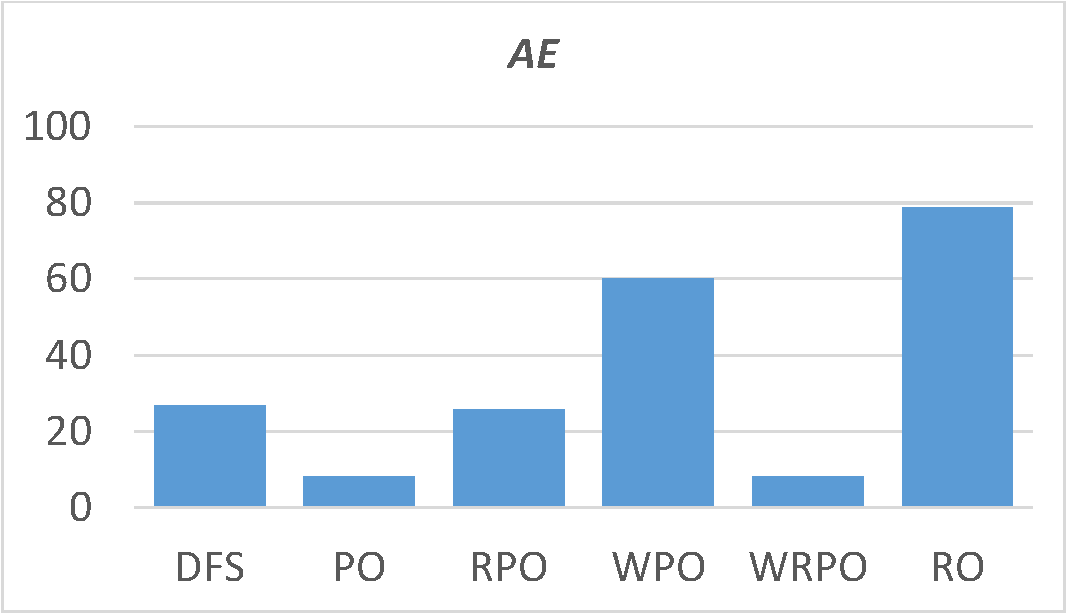
\includegraphics[width=0.32\linewidth]{ecoop-figures/ae-crop.pdf}
%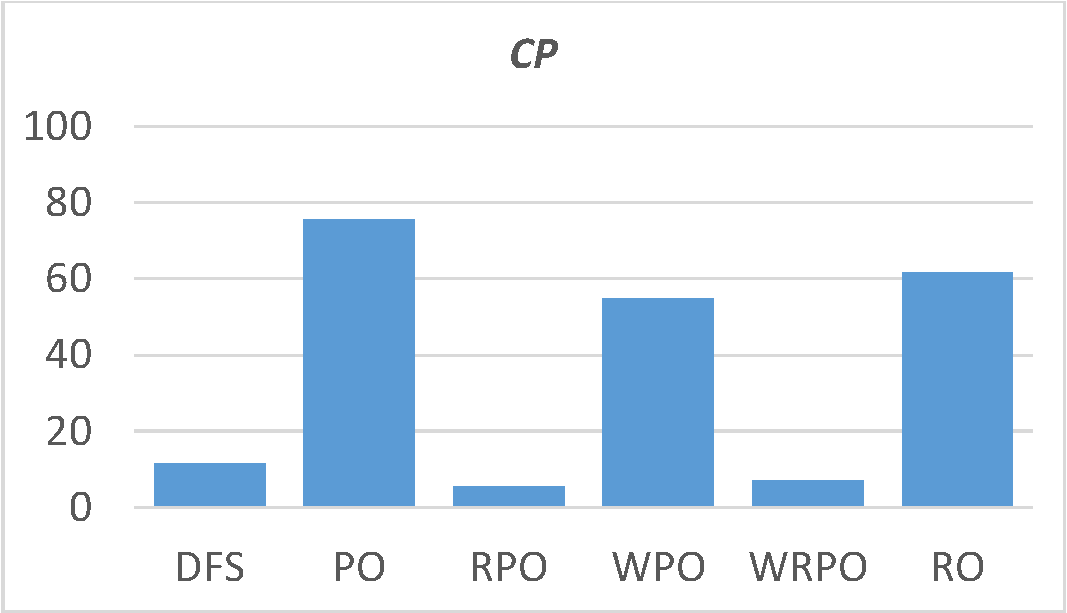
\includegraphics[width=0.32\linewidth]{ecoop-figures/cp-crop.pdf}
%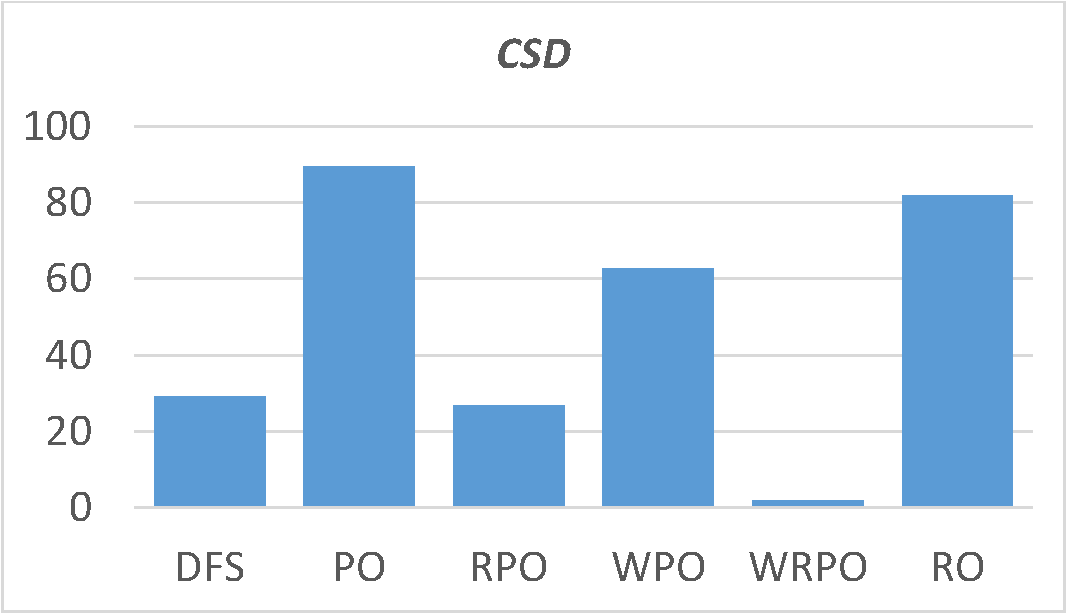
\includegraphics[width=0.32\linewidth]{ecoop-figures/csd-crop.pdf}
%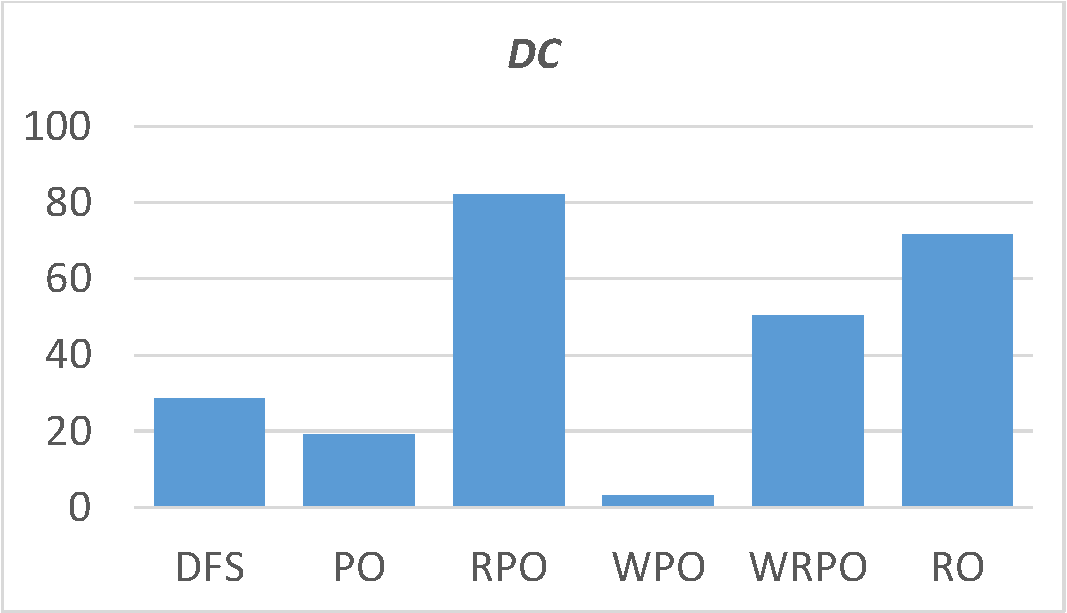
\includegraphics[width=0.32\linewidth]{ecoop-figures/dc-crop.pdf}
%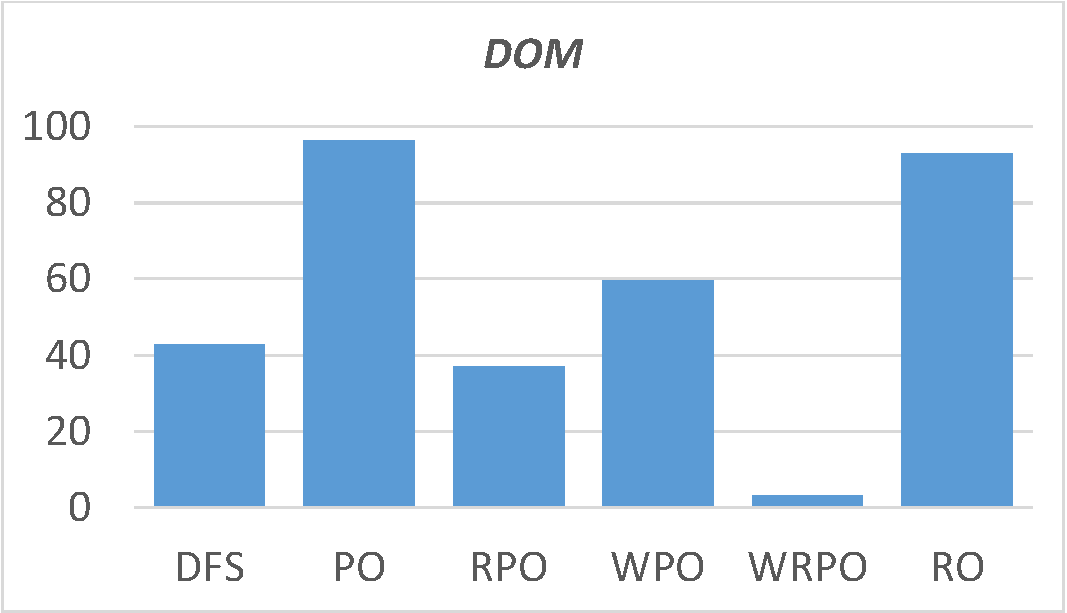
\includegraphics[width=0.32\linewidth]{ecoop-figures/dom-crop.pdf}
%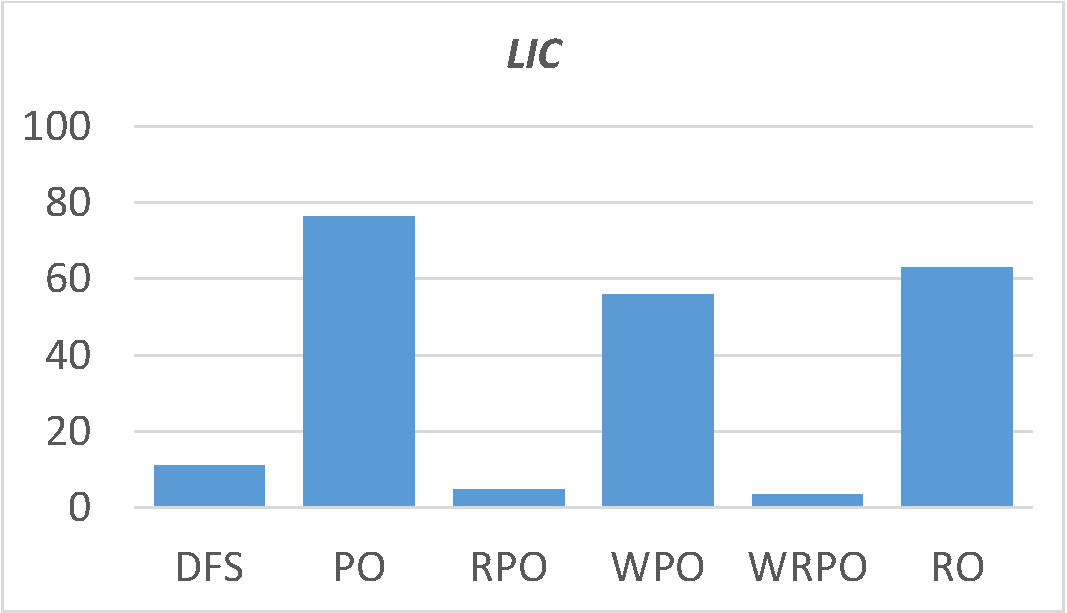
\includegraphics[width=0.32\linewidth]{ecoop-figures/lic-crop.pdf}
%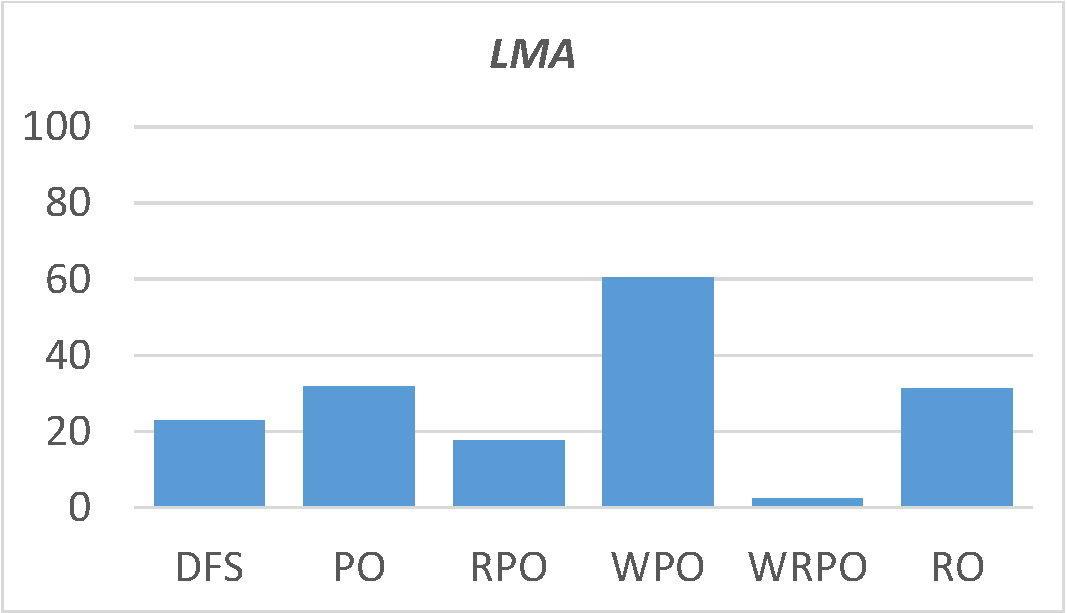
\includegraphics[width=0.32\linewidth]{ecoop-figures/lma-crop.pdf}
%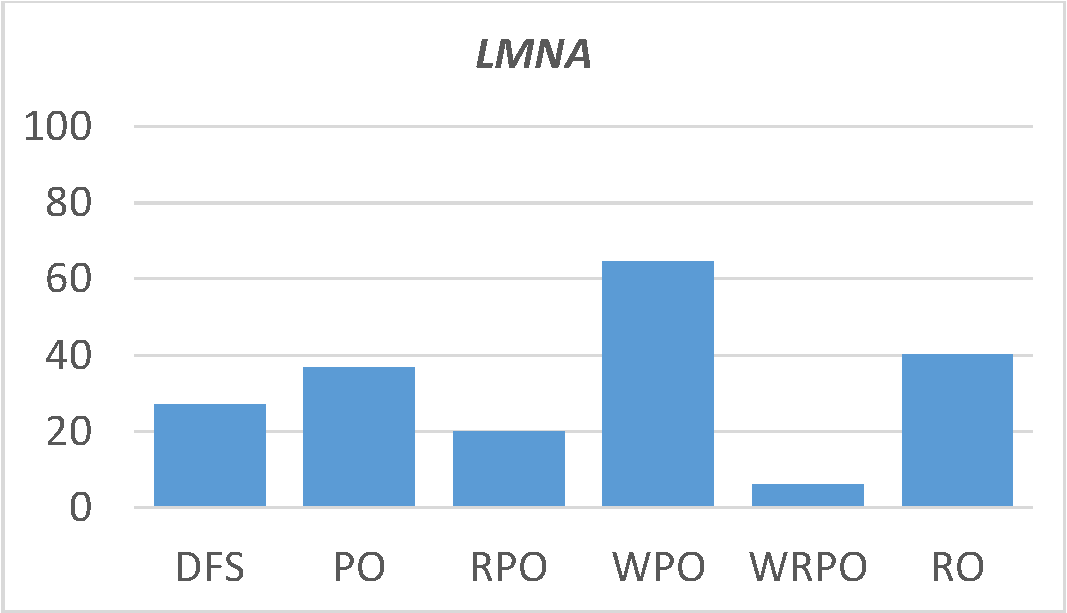
\includegraphics[width=0.32\linewidth]{ecoop-figures/lmna-crop.pdf}
%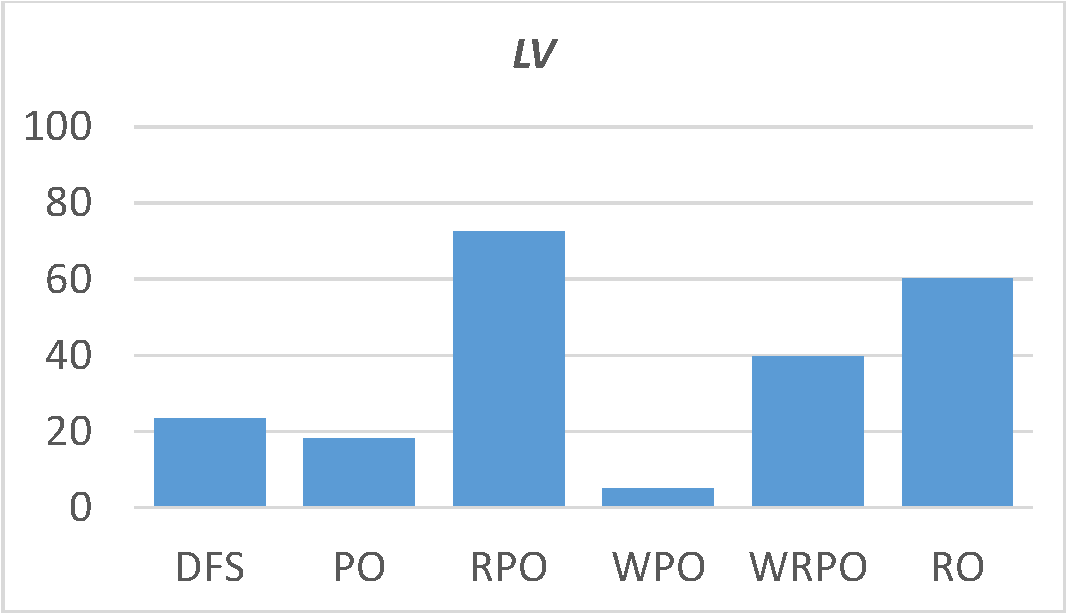
\includegraphics[width=0.32\linewidth]{ecoop-figures/lv-crop.pdf}
%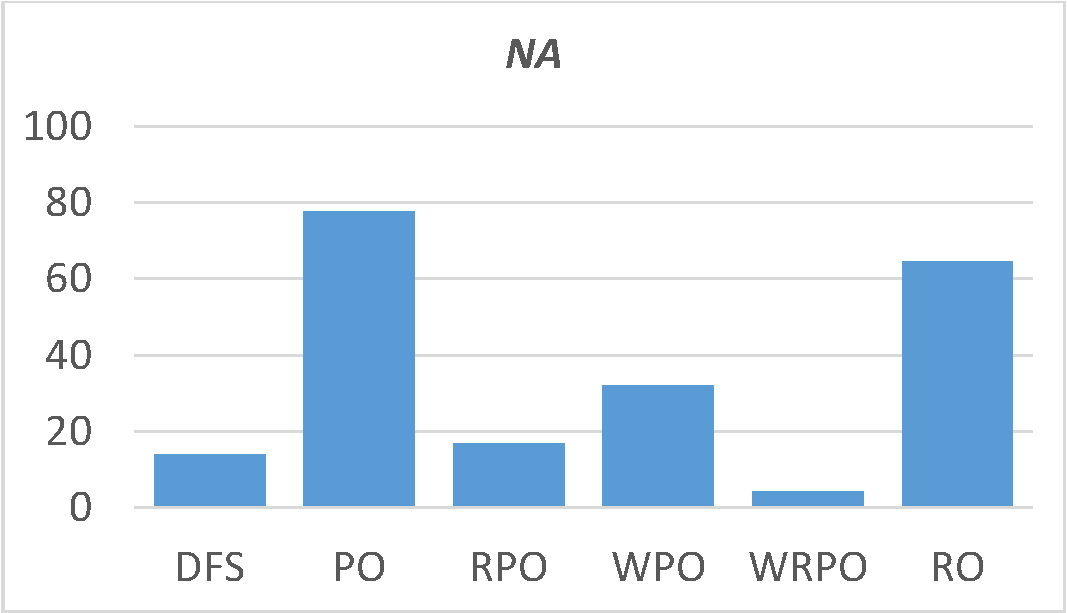
\includegraphics[width=0.32\linewidth]{ecoop-figures/na-crop.pdf}
%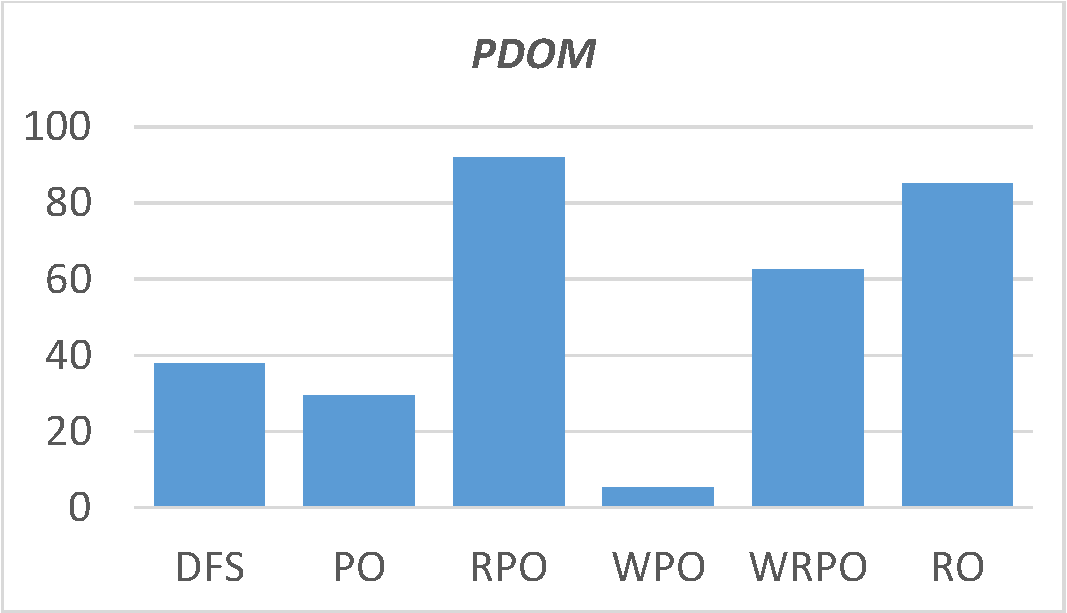
\includegraphics[width=0.32\linewidth]{ecoop-figures/pdom-crop.pdf}
%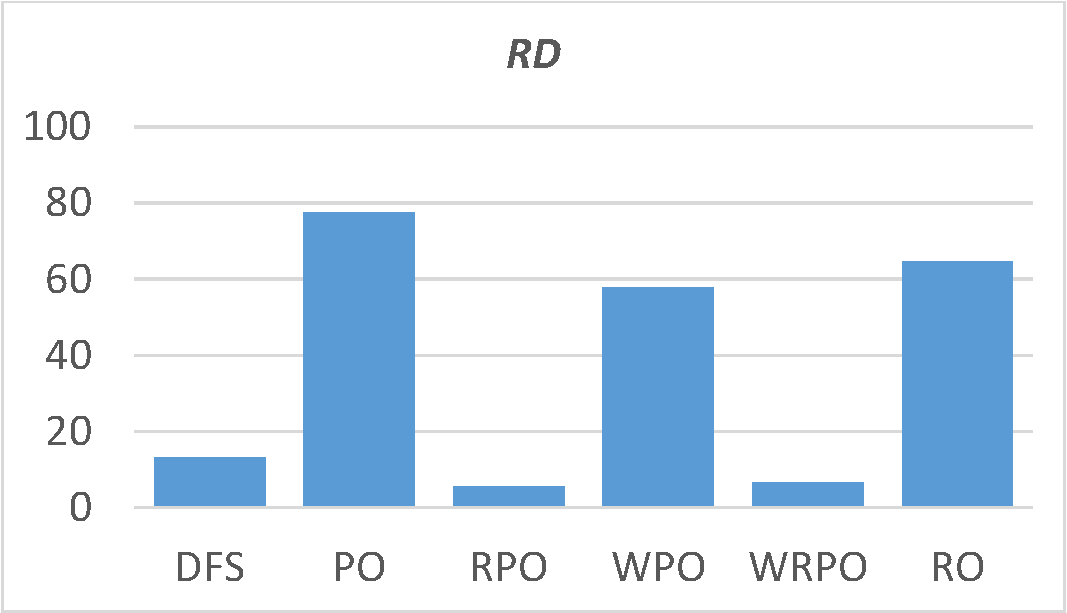
\includegraphics[width=0.32\linewidth]{ecoop-figures/rd-crop.pdf}
%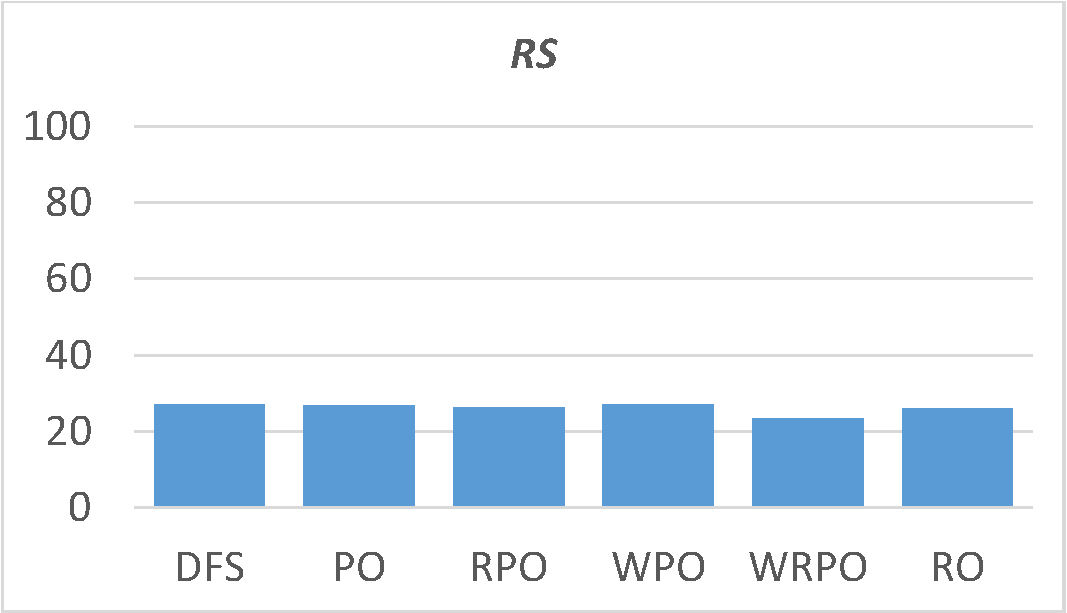
\includegraphics[width=0.32\linewidth]{ecoop-figures/rs-crop.pdf}
%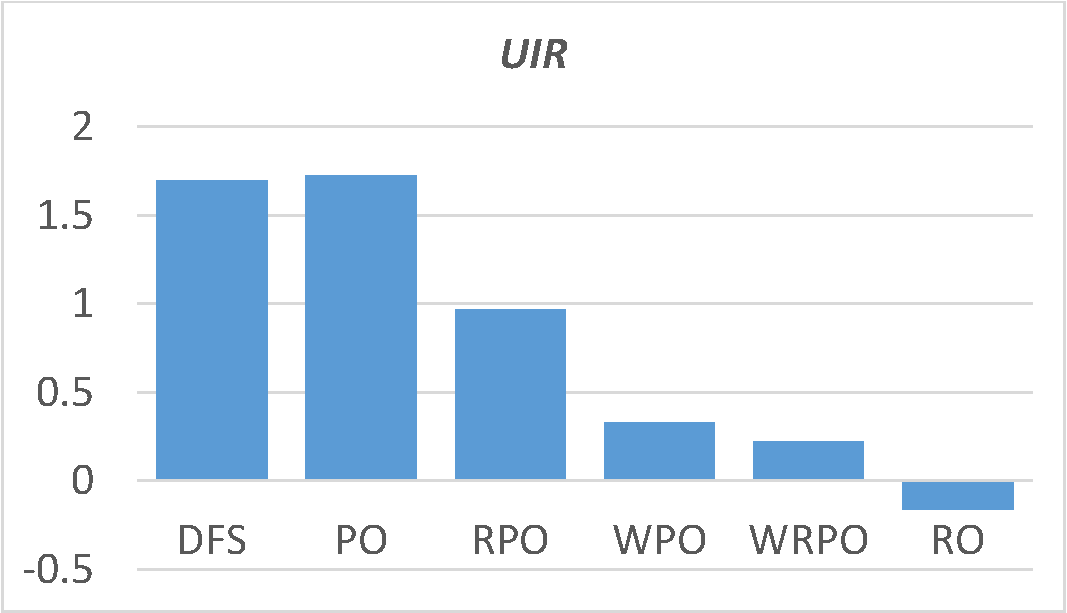
\includegraphics[width=0.32\linewidth]{ecoop-figures/uir-crop.pdf}
%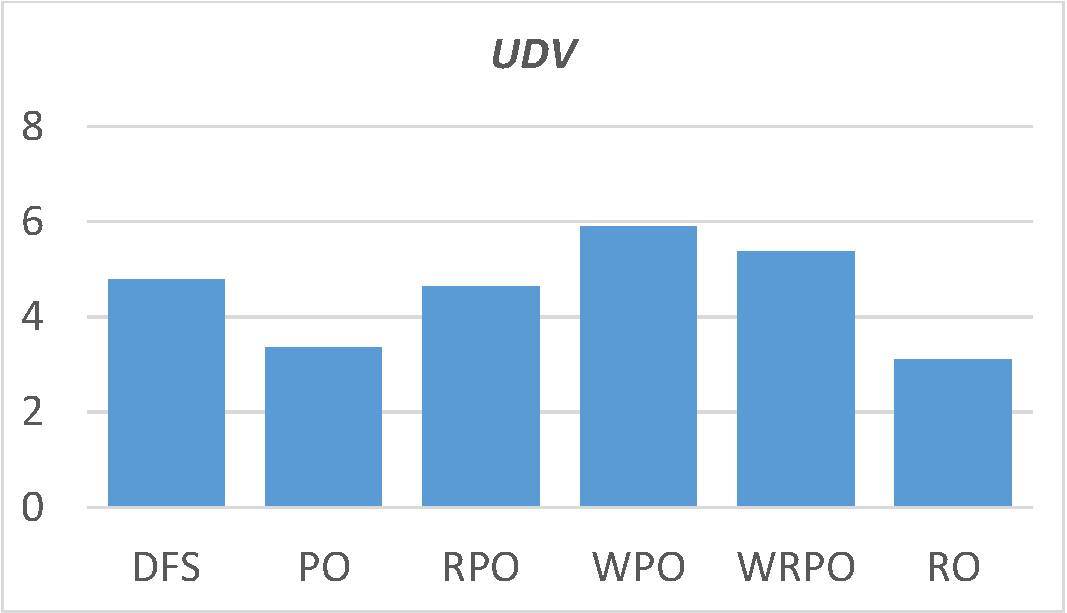
\includegraphics[width=0.32\linewidth]{ecoop-figures/udv-crop.pdf}
%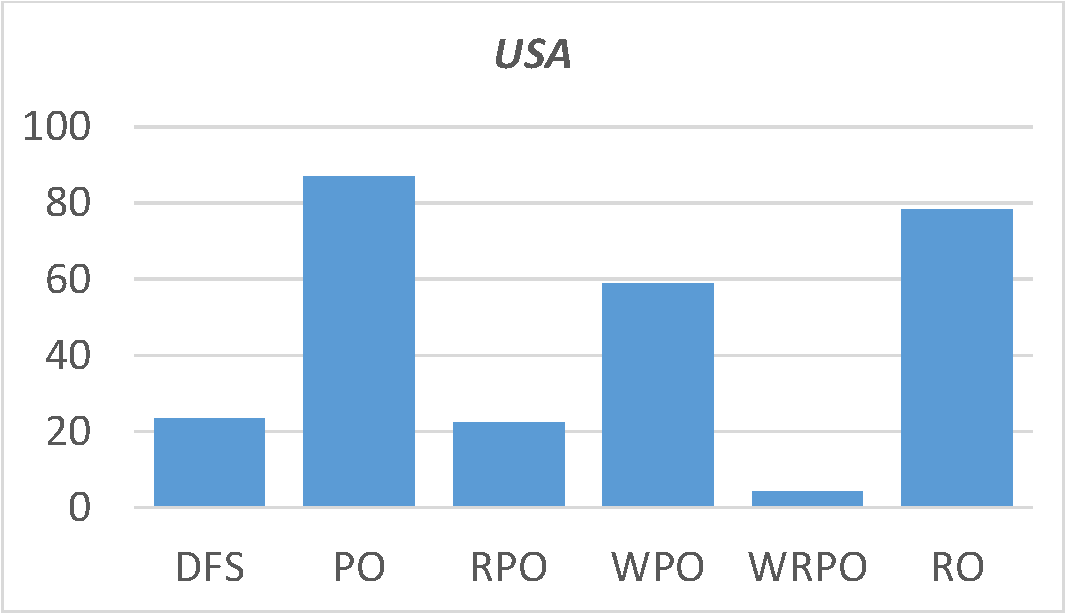
\includegraphics[width=0.32\linewidth]{ecoop-figures/usa-crop.pdf}
%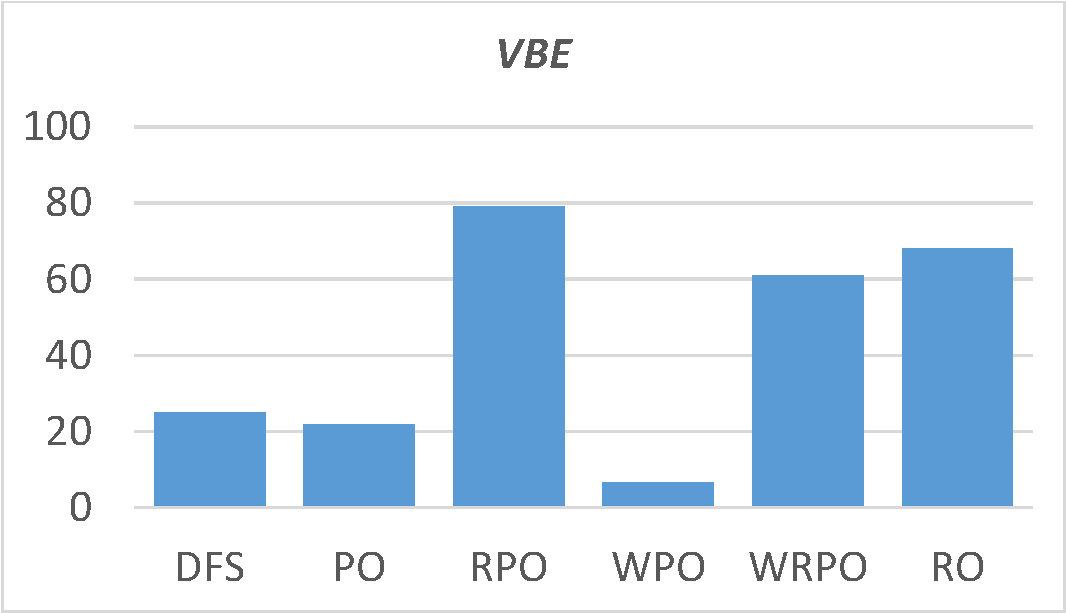
\includegraphics[width=0.32\linewidth]{ecoop-figures/vbe-crop.pdf}
%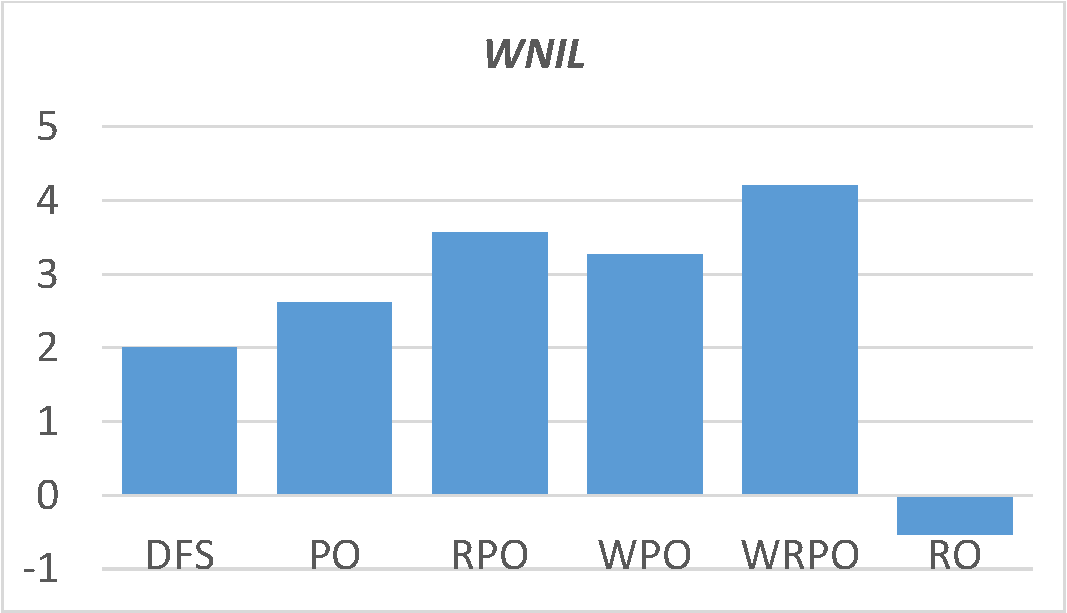
\includegraphics[width=0.32\linewidth]{ecoop-figures/wnil-crop.pdf}\newline
%\textbf{c) \textit{Overall}}\\
%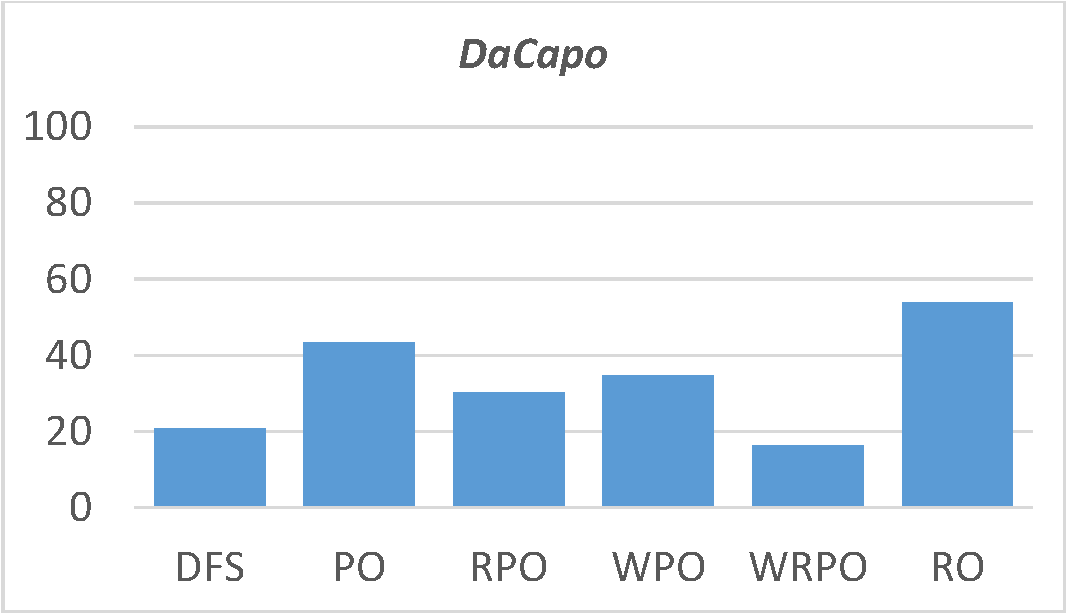
\includegraphics[width=0.32\linewidth]{ecoop-figures/dacapo-overall-crop.pdf}
  %\caption[Percentage reduction in execution time of hybrid approach over other candidate traversals on \textit{DaCapo} (Sequential mode) and \textit{SourceForge} (Cluster mode).]
%{Percentage reduction in execution time of hybrid approach over other candidate traversals on \textit{DaCapo} (Sequential mode) and \textit{SourceForge} (Cluster mode).
%\label{fig:dacapo-singlemachine-time-percentage}}
%\end{figure*}

%\begin{figure*}[ht!]
%\centering
%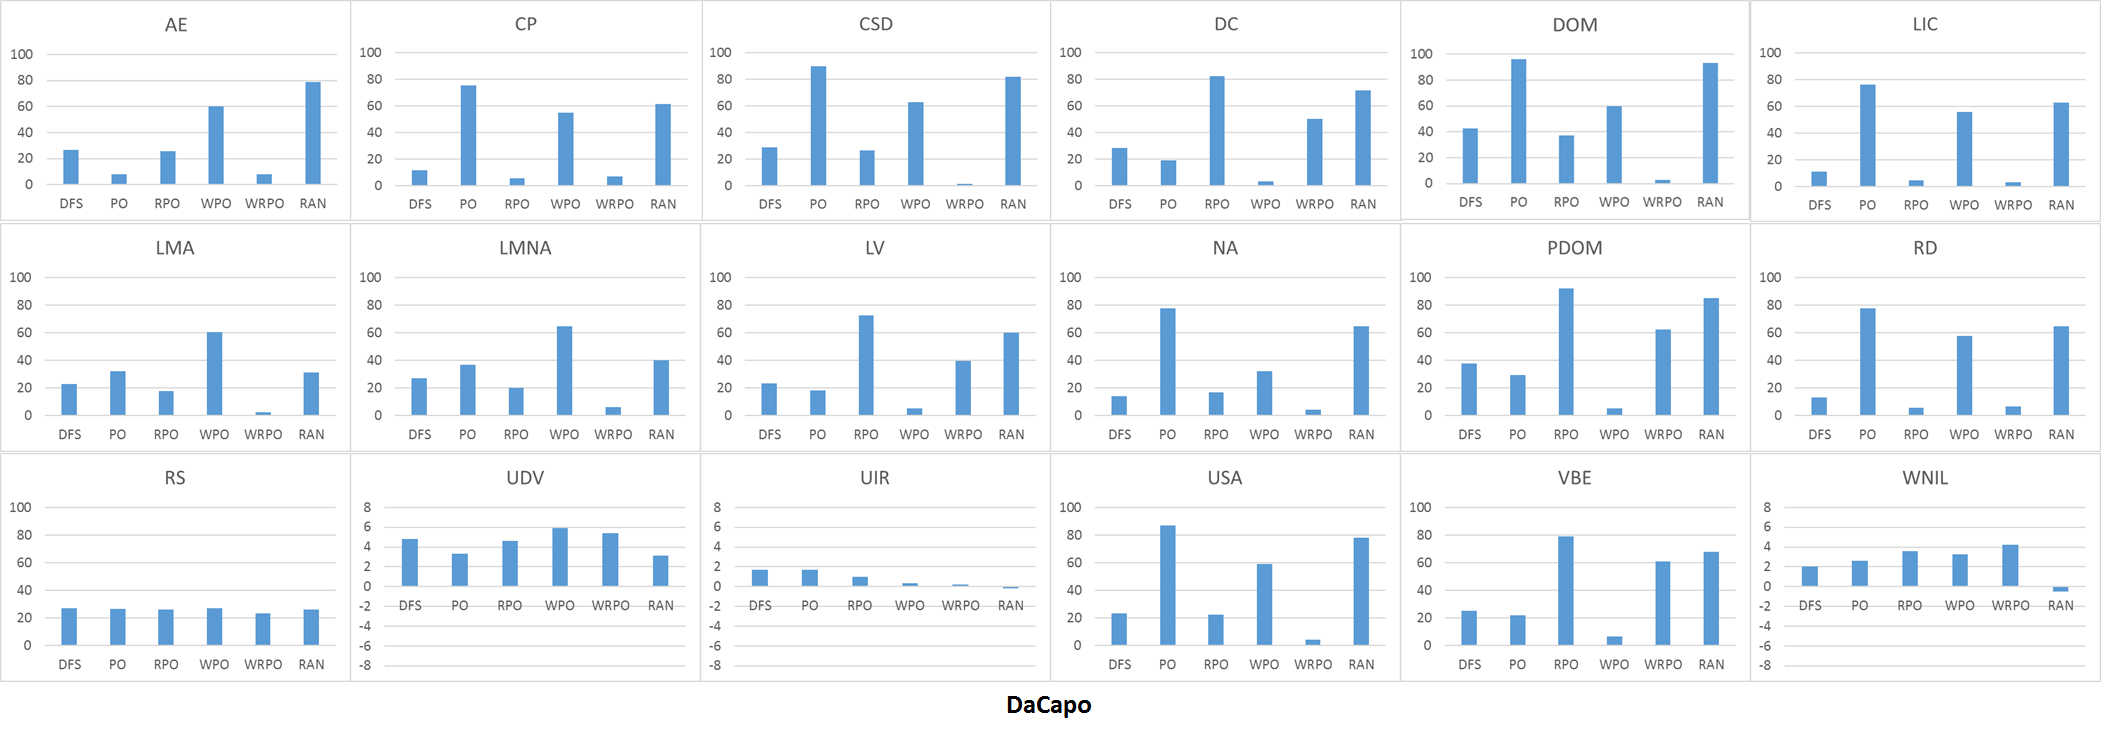
\includegraphics[width=\textwidth]{ecoop-figures/dacapo-seq-reduction.png}
%  \caption[Percentage reduction in execution time of hybrid approach over other candidate traversals on \textit{DaCapo} (Sequential mode), \textit{DaCapo} (Cluster mode), \textit{SourceForge} (Cluster mode).]
%{Percentage reduction in execution time of hybrid approach over other candidate traversals on \textit{DaCapo} (Sequential mode), \textit{DaCapo} (Cluster mode), \textit{SourceForge} (Cluster mode).
%\label{fig:dacapo-singlemachine-time-percentage}}
%\end{figure*}

\begin{figure}%
\centering
\scriptsize
\begin{tabular}{lrrrrrr|rrrrrr}
\toprule
\multicolumn{1}{l}{Analysis} & \multicolumn{1}{c|}{DaCapo}                    & \multicolumn{1}{c}{GitHub} \\
\midrule
\multicolumn{1}{l}{CP} & \cellcolor{lightblue}9\%  & \cellcolor{lightblue}5\%  \\
\multicolumn{1}{l}{CSD} & \cellcolor{lightblue}4\%  & \cellcolor{lightblack}12\% \\
\multicolumn{1}{l}{DC} & \cellcolor{lightblue}7\%  & \cellcolor{lightblue}7\%  \\
\multicolumn{1}{l}{LIC} & \cellcolor{lightblue}7\%  & \cellcolor{lightblack}19\% \\
\multicolumn{1}{l}{USA} & \cellcolor{lightblue}9\%  & \cellcolor{lightblue}9\% \\
\multicolumn{1}{l}{VFR} & \cellcolor{lightblack}15\%  & \cellcolor{lightblue}9\% \\
\multicolumn{1}{l}{MWN} & \cellcolor{lightblack}15\%  & \cellcolor{lightblue}9\% \\
\multicolumn{1}{l}{AE} & \cellcolor{lightblack}14\%  &  \cellcolor{lightblack}11\% \\
\multicolumn{1}{l}{DOM} & \cellcolor{lightblue}6\%  & \cellcolor{lightblue}6\% \\
\multicolumn{1}{l}{LMA} & \cellcolor{lightblue}6\%  & \cellcolor{lightblue}6\% \\
\multicolumn{1}{l}{LMNA} & \cellcolor{lightblue}9\%  & \cellcolor{lightblue}7\% \\
\multicolumn{1}{l}{LV} & \cellcolor{lightblack}11\%  & \cellcolor{lightblack}11\%  \\
\multicolumn{1}{l}{NA} & \cellcolor{lightblack}10\%  & \cellcolor{lightblack}10\%  \\
\multicolumn{1}{l}{PDOM} & \cellcolor{lightblack}10\%  & \cellcolor{lightblack}24\% \\
\multicolumn{1}{l}{RD} & \cellcolor{lightblue}9\%  & \cellcolor{lightblue}5\% \\
\multicolumn{1}{l}{RS} & \cellcolor{lightblack}28\%  & \cellcolor{lightblue}7\% \\
\multicolumn{1}{l}{VBE} & \cellcolor{lightblack}13\%  & \cellcolor{lightblack}10\% \\
\multicolumn{1}{l}{SS} & \cellcolor{lightblack}22\%  & \cellcolor{lightblack}10\%  \\
\multicolumn{1}{l}{UDV} &  \cellcolor{lightblue}3\%   &  \cellcolor{lightblue}0\%  \\
\multicolumn{1}{l}{UIR} &  \cellcolor{lightblue}0\%   &  \cellcolor{lightblue}0\%  \\
\multicolumn{1}{l}{WNIL} &  \cellcolor{lightblue}2\%   &  \cellcolor{lightblue}0\% \\
\bottomrule
\end{tabular}%
\caption{Reduction in running times against hand optimized analysis.}
\label{fig:reduction-oopsla}
\end{figure}


Another way to extract more performance is to hand optimize the analysis.
\fignref{fig:reduction-oopsla} compares Hybrid approach against hand optimized analysis. Hand optimized analysis has single best optimized traversal strategy applied for each analysis. For data-flow analysis, hand optimized analysis uses WPO/WRPO guideline while for non data flow analysis, it uses ANY traversal strategy, as it is the best traversal strategy for non data-flow analysis. WPO/WRPO guideline suggests that if the direction of the traversal is backward, use WPO else use WRPO. This guideline  
simplifies the hybrid approach, where the decision is based on only traversal 
direction while Hybrid approach uses the decision tree in \fignref{fig:decision-diagram}. 
\fignref{fig:reduction-oopsla} shows the 
comparison of hybrid approach against hand optimized analysis. We can see that for 
about half of the data-flow analysis, we gain at least 10\% reduction. For analysis like 
RS, SS, VFR and MWN, the gain is much higher since these analyses are 
selective in terms of the program statements that they analyze. WPO and WRPO 
would not work for these analyses since in case of both WPO and WRPO, there 
exists a fixed cost of creating and maintaining a worklist of size equals to 
the number of CFG nodes. When analyses selectively analyzes a small subset of 
all nodes in the CFGs, this overhead becomes substantial. Our hybrid strategy 
is not only able to select an alternative strategy instead of WPO/WRPO for 
such selective analyses, whenever possible (when the input graphs do not 
contain loops), but also optimize WPO/WRPO (in case of input graphs with loops), 
such that the overheads are minimized.
For non-data flow analysis, there is no gain against hand optimized analysis since ANY is the best traversal strategy for such analysis and both Hybrid approach and hand optimized analysis applied ANY traversal strategy for all the graphs for non-data flow analysis.
\chapter{Correctness of Analysis Results}
\label{sec:soundness}

To evaluate the correctness of analysis results, we first chose worklist 
as standard strategy to run analyses on DaCapo dataset to create the 
groundtruth of the results. We then ran analyses using our hybrid approach 
and compared the results with the groundtruth. In all analyses on all 
input graphs from the dataset, the results from our hybrid approach always 
exactly matched the corresponding ones in the groundtruth. 
%\todo{That means the 
%hybrid approach does not compromise on the correctness of the result while 
%picking and optimizing the best traversal strategy.} 

\chapter{Traversal Strategy Selection Precision}
\label{sec:prediction-accuracy}

% Table generated by Excel2LaTeX from sheet 'Sheet1'
\begin{table}
\footnotesize
\centering
\caption{Traversal strategy prediction precision.}
\setlength{\tabcolsep}{2pt}
\begin{tabular}{cr}
\toprule
Analysis & Precision \\
\midrule
DOM, PDOM, WNIL, UDV, UIR & 100.00\% \\
CP, CSD, DC, LIC, USA, VFR, MWN, AE, LMA, LMNA, LV, NA, RD, RS, VBE, SS  & 99.99\% \\
\bottomrule
\end{tabular}%
\label{tab:prediction-precision}%
\end{table}%

\begin{figure}[h]
\centering
\subfloat[CP]{
\fbox{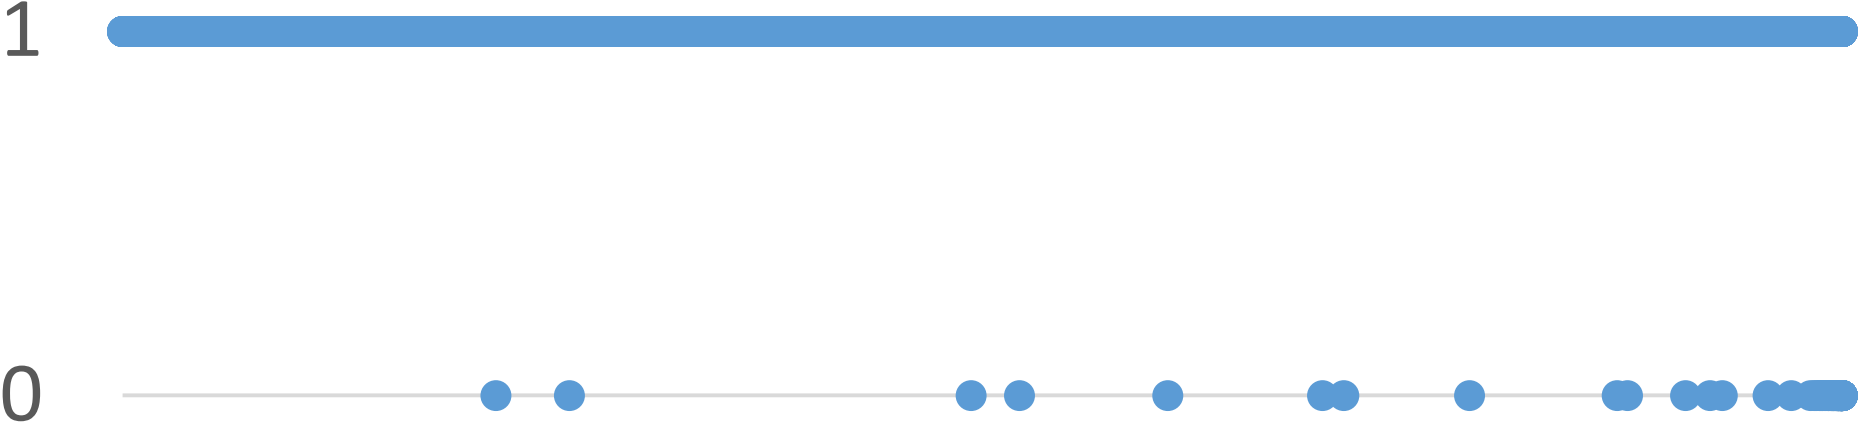
\includegraphics[width=0.22\linewidth]{figures/loop-cp.png}}
\label{fig:loop-cp}
}
\subfloat[CSD]{
\fbox{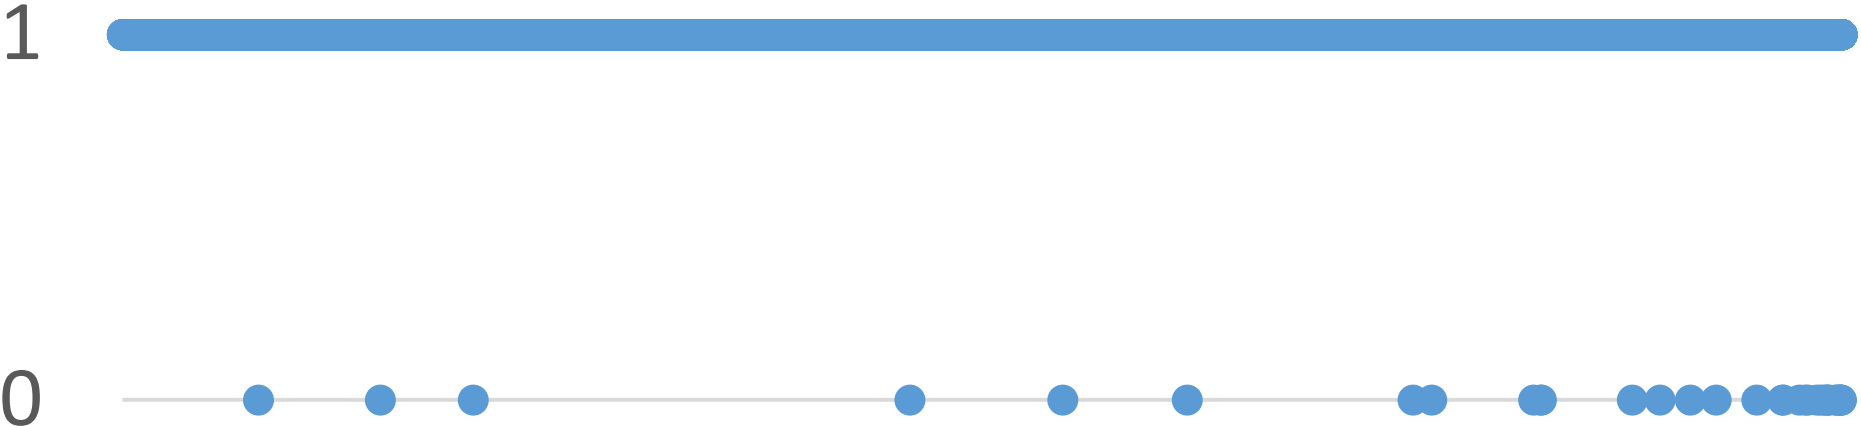
\includegraphics[width=0.22\linewidth]{figures/loop-csd.png}}
\label{fig:loop-csd}
}
\subfloat[DC]{
\fbox{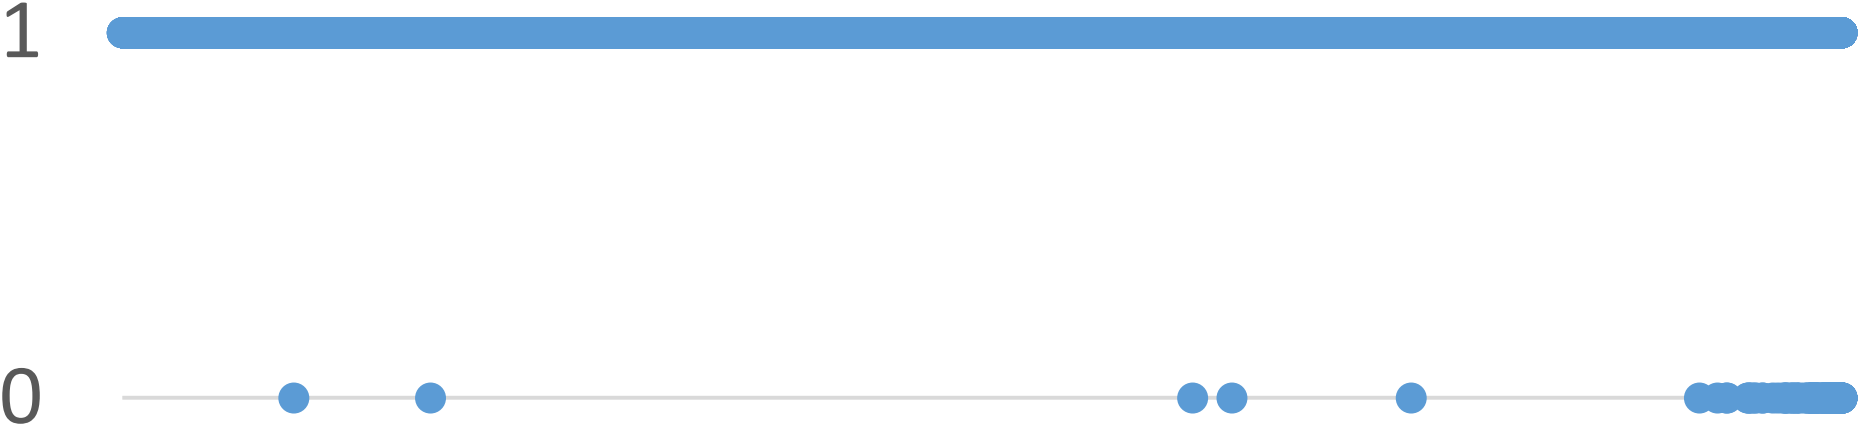
\includegraphics[width=0.22\linewidth]{figures/loop-dc.png}}
\label{fig:loop-dc}
}
\subfloat[LIC]{
\fbox{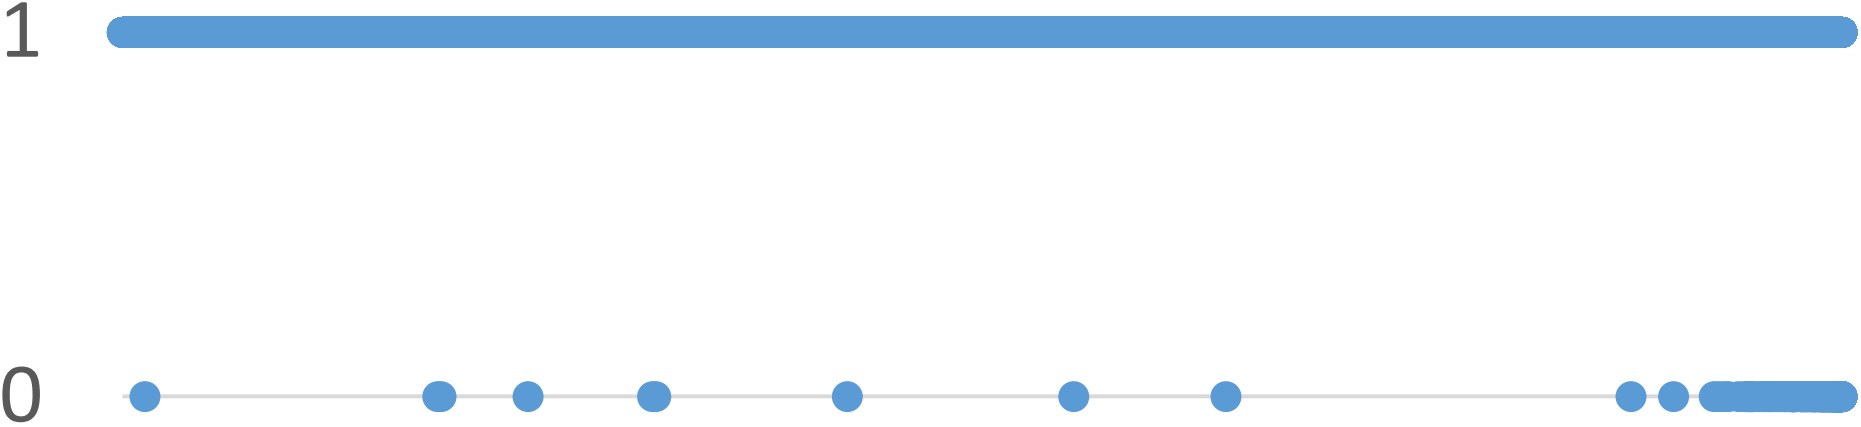
\includegraphics[width=0.22\linewidth]{figures/loop-lic.png}}
\label{fig:loop-lic}
}\\
\subfloat[USA]{
\fbox{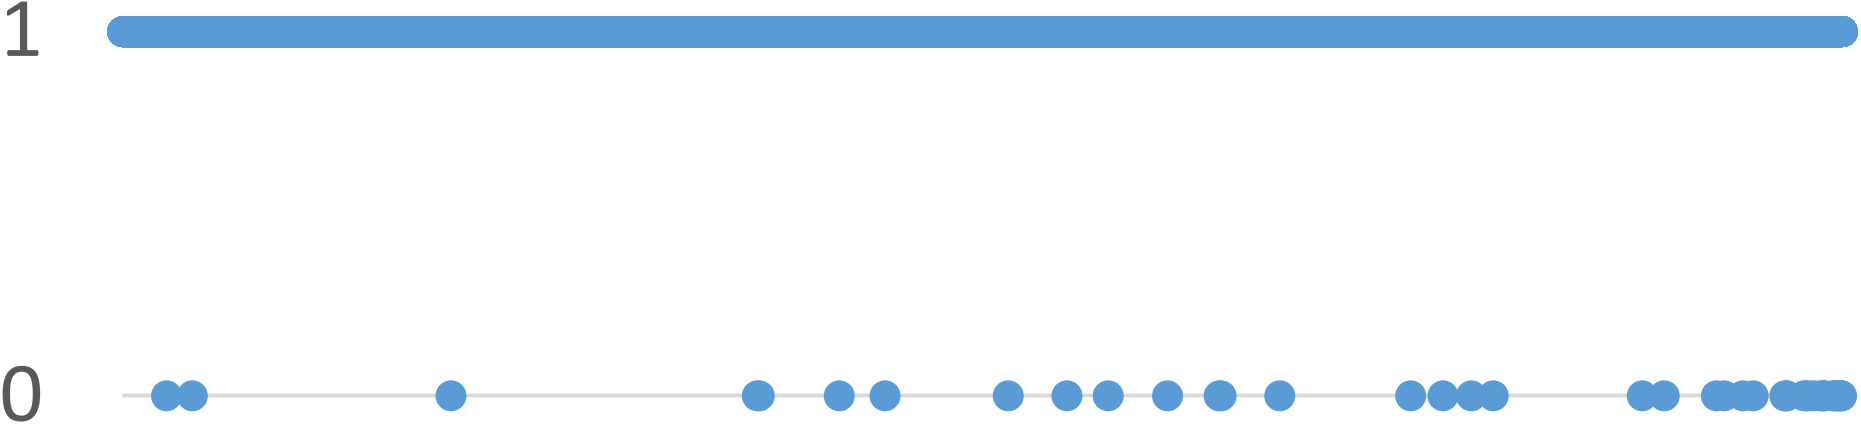
\includegraphics[width=0.22\linewidth]{figures/loop-usa.png}}
\label{fig:loop-use}
}
\subfloat[VFR]{
	\fbox{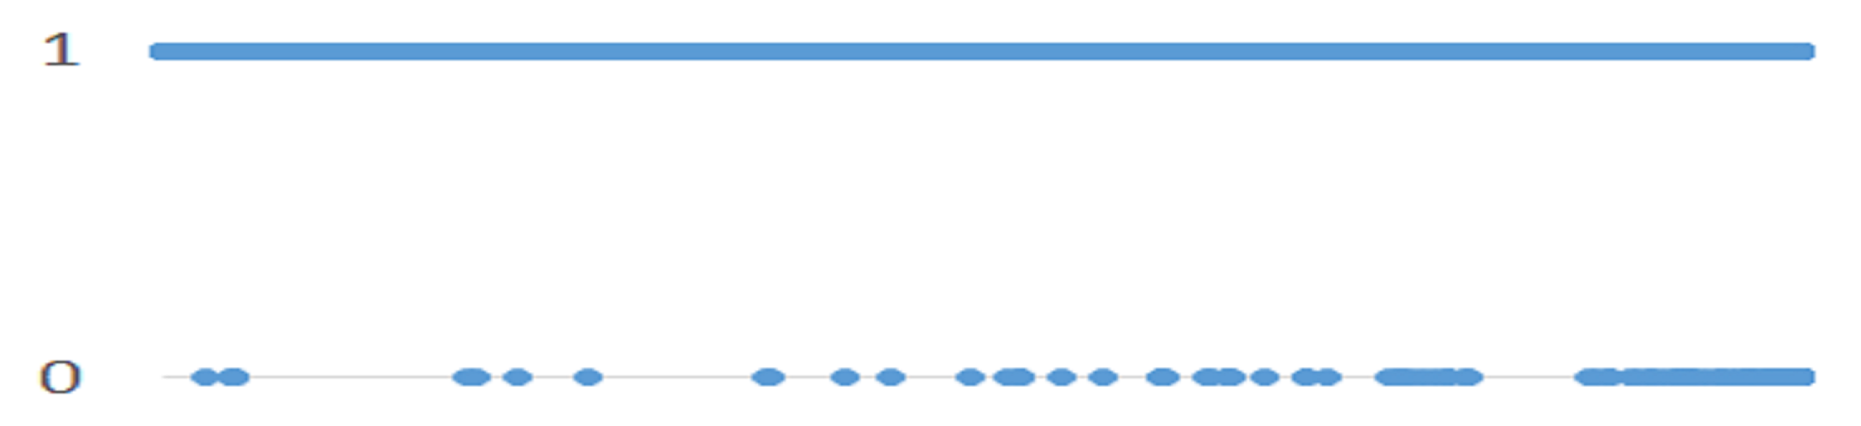
\includegraphics[width=0.22\linewidth]{figures/loop-vfr.png}}
	\label{fig:loop-vfr}
}
\subfloat[MWN]{
	\fbox{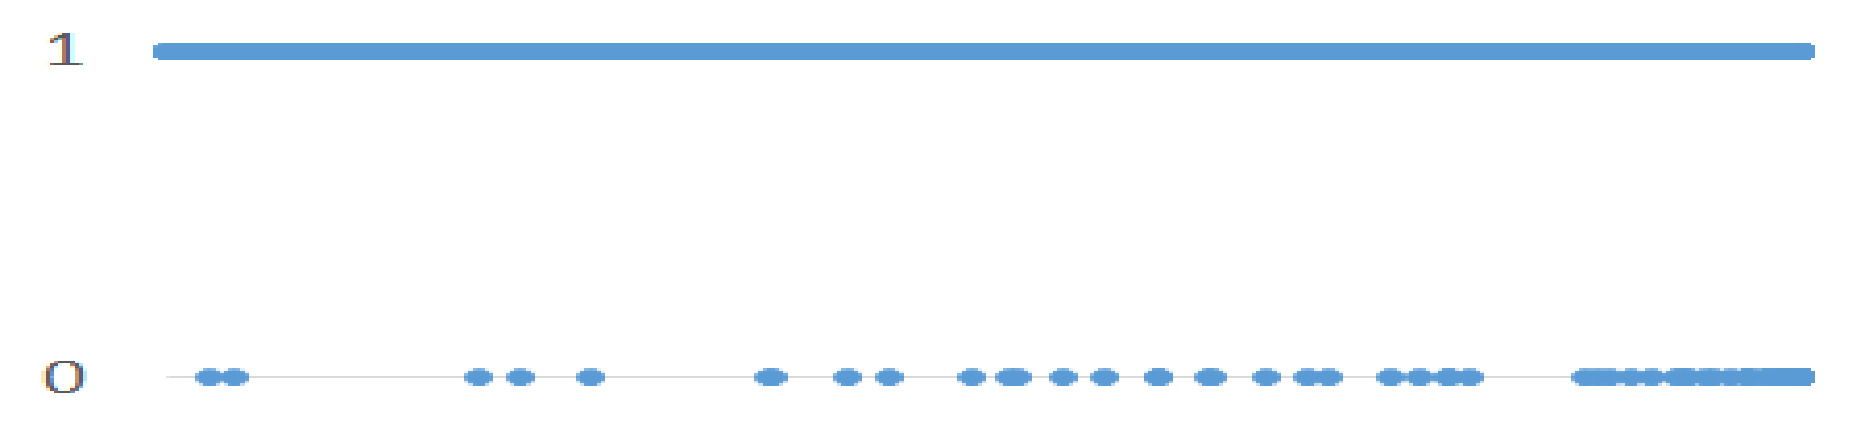
\includegraphics[width=0.22\linewidth]{figures/loop-mwn.png}}
	\label{fig:loop-mwn}
}
\subfloat[AE]{
\fbox{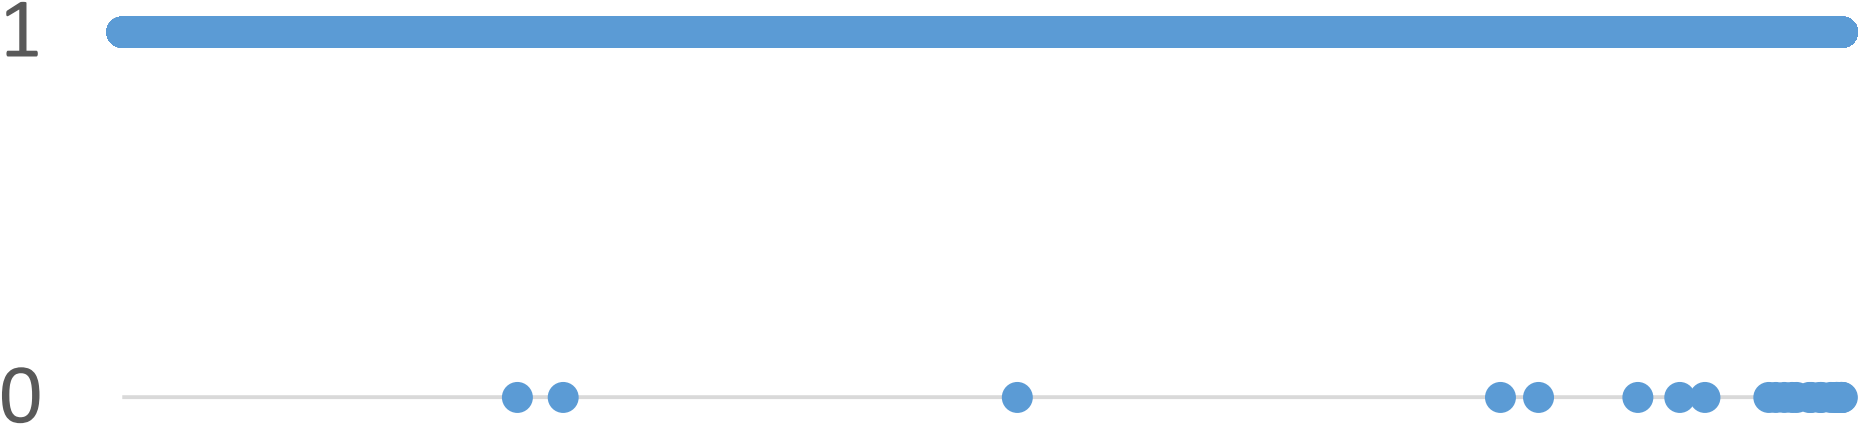
\includegraphics[width=0.22\linewidth]{figures/loop-ae.png}}
\label{fig:loop-ae}
}\\
\subfloat[LMA]{
\fbox{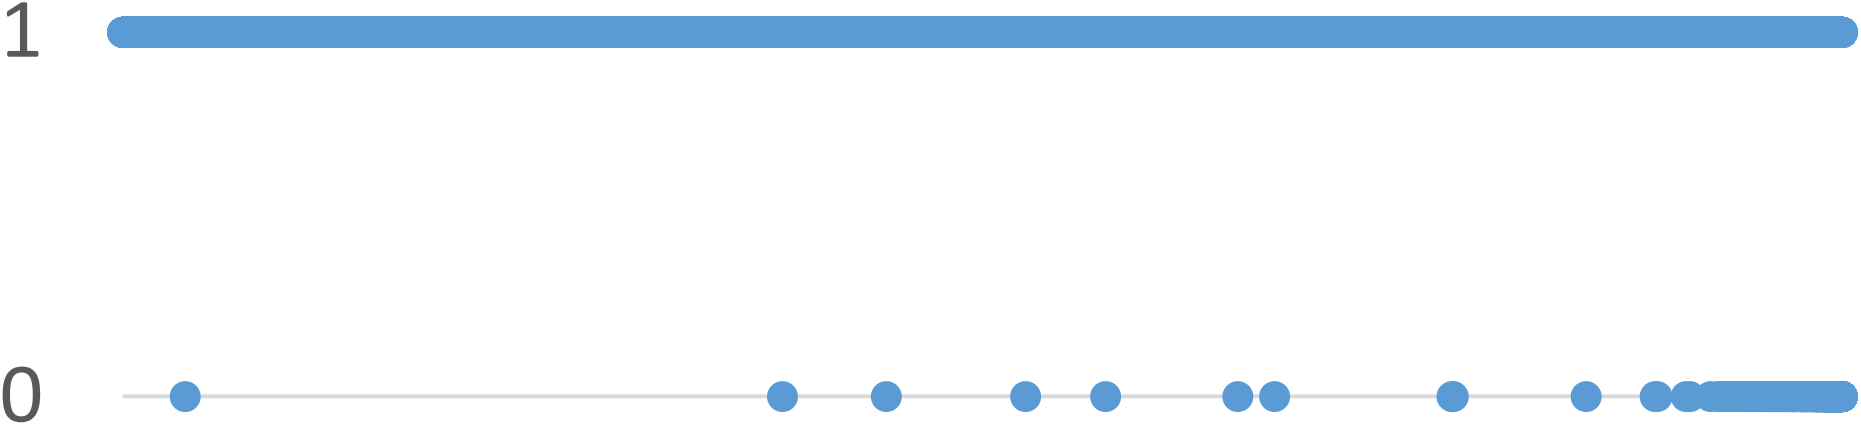
\includegraphics[width=0.22\linewidth]{figures/loop-lma.png}}
\label{fig:loop-lma}
}
\subfloat[LMNA]{
\fbox{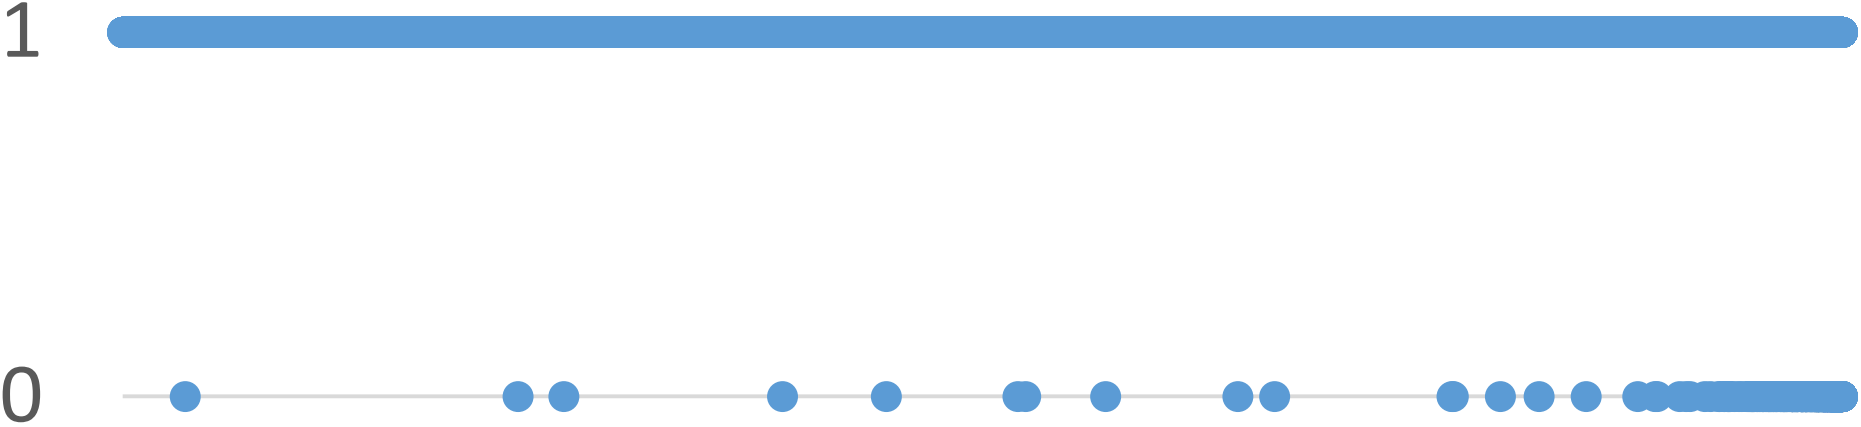
\includegraphics[width=0.22\linewidth]{figures/loop-lmna.png}}
\label{fig:loop-lmna}
}
\subfloat[LV]{
\fbox{\includegraphics[width=0.22\linewidth]{figures/loop-lv.png}}
\label{fig:loop-lv}
}
\subfloat[NA]{
\fbox{\includegraphics[width=0.22\linewidth]{figures/loop-na.png}}
\label{fig:loop-na}
}\\
\subfloat[RD]{
\fbox{\includegraphics[width=0.22\linewidth]{figures/loop-rd.png}}
\label{fig:loop-rd}
}
\subfloat[RS]{
\fbox{\includegraphics[width=0.22\linewidth]{figures/loop-rs.png}}
\label{fig:loop-rs}
}
\subfloat[VBE]{
\fbox{\includegraphics[width=0.22\linewidth]{figures/loop-vbe.png}}
\label{fig:loop-vbe}
}
\subfloat[SS]{
	\fbox{\includegraphics[width=0.22\linewidth]{figures/loop-ss.png}}
	\label{fig:loop-ss}
}\\
\caption{Scatter charts for analyses that have loop sensitive traversals. 
%$x$-axis lists the CFGs in the increasing of the node size. 
}
\label{fig:loops}
\end{figure}



In this experiment, we evaluated how well the hybrid approach picks the most 
time-efficient strategy. We ran the 21 analyses on the DaCapo dataset using 
all the candidate traversals and the one selected by the hybrid approach. One 
selection is counted for each pair of a traversal and an input graph where 
the hybrid approach selects a traversal strategy based on the properties of 
the analysis and input graph. A selection is considered correct if its 
running time is at least as good as the running time of the fastest among all 
candidates. The precision is computed as the ratio between the number of 
correct selections over the total number of all selections. 
%
As shown in \tabref{tab:prediction-precision}, the selection precision is 100\% 
for all analyses that are not \textit{loop sensitive}. For analyses that 
involve \textit{loop sensitive} traversals, the prediction precision is 99.99\%. 

We further analyzed the result to see what contributed to these mispredictions. 
Let us break the CFGs in the DaCapo dataset by the graph \graphprop{}: sequential CFGs, 
CFGs with branches and no loops, and CFGs with loops, and discuss the selection precision.

For \textbf{sequential CFGs \& CFGs with branches and no loops}, the selection  
precision is 100\%---the hybrid approach always picks the most time-efficient 
traversal strategy.

For \textbf{CFGs with loops}, the selection precision is 100\% for \emph{loop 
	insensitive} traversals. The mispredictions occur with \emph{loop sensitive} 
traversals on CFGs with loops. Figure \ref{fig:loops} shows scatter charts 
for the traversal selection results for 16 analyses that are \textit{loop 
	sensitive}. In the chart, 1 indicates a correct selection and 0 indicates a 
misprediction. CFGs are organized along the $x$- axis in the increasing order 
of their sizes measured as the numbers of nodes. 
%
The scatter charts show that the mispredictions tend to happen with larger 
CFGs. 
%
The reason is that, for \textit{loop sensitive} traversals, the hybrid 
approach picks worklist as the best strategy. The worklist approach was 
picked because it visits only as many nodes as needed when compared to other 
traversal strategies which visit redundant nodes. However using worklist 
imposes an overhead of creating and maintaining a worklist containing all 
nodes in the CFG. This overhead is negligible for small CFGs. However, when 
running analyses on large CFGs, this overhead could become higher 
than the cost for visiting redundant nodes. Therefore, selecting worklist for 
\emph{loop sensitive} traversals on large CFGs might not always result in the 
best running times. 

\begin{figure}[h]
\centering

\includegraphics[width=0.32\linewidth]{tex-figures/misprediction/cp-crop.pdf}
\label{fig:mis-cp}
\includegraphics[width=0.32\linewidth]{tex-figures/misprediction/csd-crop.pdf}
\label{fig:mis-csd}
\includegraphics[width=0.32\linewidth]{tex-figures/misprediction/DC-crop.pdf}
\label{fig:mis-dc}
\\
\includegraphics[width=0.32\linewidth]{tex-figures/misprediction/LIC-crop.pdf}
\label{fig:mis-lic}
\includegraphics[width=0.32\linewidth]{tex-figures/misprediction/usa-crop.pdf}
\label{fig:mis-use}
	\includegraphics[width=0.32\linewidth]{tex-figures/misprediction/vfr-crop.pdf}
	\label{fig:mis-vfr}
	\\
	\includegraphics[width=0.32\linewidth]{tex-figures/misprediction/mwn-crop.pdf}
	\label{fig:mis-mwn}
\includegraphics[width=0.32\linewidth]{tex-figures/misprediction/AE-crop.pdf}
\label{fig:mis-ae}
\includegraphics[width=0.32\linewidth]{tex-figures/misprediction/LMA-crop.pdf}
\label{fig:mis-lma}
\\
\includegraphics[width=0.32\linewidth]{tex-figures/misprediction/LMNA-crop.pdf}
\label{fig:mis-lmna}
\includegraphics[width=0.32\linewidth]{tex-figures/misprediction/LV-crop.pdf}
\label{fig:mis-lv}
\includegraphics[width=0.32\linewidth]{tex-figures/misprediction/NA-crop.pdf}
\label{fig:mis-na}
\\
\includegraphics[width=0.32\linewidth]{tex-figures/misprediction/rd-crop.pdf}
\label{fig:mis-rd}
\includegraphics[width=0.32\linewidth]{tex-figures/misprediction/rs-crop.pdf}
\label{fig:mis-rs}
\includegraphics[width=0.32\linewidth]{tex-figures/misprediction/VBE-crop.pdf}
\label{fig:mis-vbe}
\\
	\includegraphics[width=0.32\linewidth]{tex-figures/misprediction/SS-crop.pdf}
	\label{fig:mis-ss}
\caption{Hybrid approach's performance against best approaches for mis-predicted graphs.}
\label{fig:mis-graph}
\end{figure}


%\begin{figure}
%	\centering
%	\includegraphics[width=0.50\linewidth]{tex-figures/loop-ae-ns.pdf}
%	\caption{Hybrid approach's performance against best approaches for mis-predicted graphs.}%
%	\label{fig:loop-ae-ns}%
%\end{figure}

\fignref{fig:mis-graph} shows the Hybrid approach's performance against best 
approaches for mis-predicted graphs for 16 analyses that has \emph{loop sensitive} traversals. We can see that for 
majority of the mis-predicted graphs, Hybrid approach's performance is 
comparable to the best approaches. For analyses like CP, CSD, LIC, USA, DC, LMA, AE, LMNA, VBE and RD, Hybrid running time are almost similar to the Best traversal strategy for smaller graphs. For graphs of size greater than 200, Hybrid starts to perform worse (1.5x - 2x) than the best traversal strategy. But for analyses like MWN, VFR, LV, NA, RS and SS, Hybrid performs worse even for smaller graphs that were mis-predicted. This is because of the complexity of the analyses. Since these analyses are lesser in complexity, even for small graphs that are mis-predicted, hybrid's performance is worse. This is because hybrid chooses Worklist for these mis-predicted analyses and in these analyses, time to maintain the Worklist is much higher than the analyses itself.
%As graph's size increases, Hybrid's performance for mis-predicted graphs worsens and is no more comparable to the best approach. 

\chapter{Analysis on the Decision Tree Distribution}
\label{sec:analysis-decision-tree}

\begin{figure*}
	\centering
	\scriptsize
\begin{tabular}{lrrrrrrrrrrr}
\toprule
      & P1    & P2    & P3    & P4    & P5    & P6    & P7    & P8    & P9    & P10   & P11 \\
\midrule
CP    & \cellcolor{lightgreen}35\%   & \cellcolor{lightred}0\%   & \cellcolor{lightgreen}10\%   & \cellcolor{lightred}0\%   & \cellcolor{lightred}0\%   & \cellcolor{lightred}0\%   & \cellcolor{lightred}0\%   & \cellcolor{lightred}0\%   & \cellcolor{lightblack}5\%   & \cellcolor{lightred}0\%   & \cellcolor{lightgreen}50\% \\
CSD   & \cellcolor{lightgreen}35\%   & \cellcolor{lightred}0\%   & \cellcolor{lightgreen}10\%   & \cellcolor{lightred}0\%   & \cellcolor{lightred}0\%   & \cellcolor{lightred}0\%   & \cellcolor{lightred}0\%   & \cellcolor{lightred}0\%   & \cellcolor{lightblack}5\%   & \cellcolor{lightred}0\%   & \cellcolor{lightgreen}50\% \\
DC    & \cellcolor{lightred}0\%   & \cellcolor{lightgreen}35\%   & \cellcolor{lightred}0\%   & \cellcolor{lightgreen}10\%   & \cellcolor{lightred}0\%   & \cellcolor{lightred}0\%   & \cellcolor{lightred}0\%   & \cellcolor{lightred}0\%   & \cellcolor{lightred}0\%   & \cellcolor{lightblack}5\%   & \cellcolor{lightgreen}50\% \\
LIC   & \cellcolor{lightgreen}35\%   & \cellcolor{lightred}0\%   & \cellcolor{lightgreen}10\%   & \cellcolor{lightred}0\%   & \cellcolor{lightred}0\%   & \cellcolor{lightred}0\%   & \cellcolor{lightred}0\%   & \cellcolor{lightred}0\%   & \cellcolor{lightblack}5\%   & \cellcolor{lightred}0\%   & \cellcolor{lightgreen}50\% \\
USA   & \cellcolor{lightgreen}35\%   & \cellcolor{lightred}0\%   & \cellcolor{lightgreen}10\%   & \cellcolor{lightred}0\%   & \cellcolor{lightred}0\%   & \cellcolor{lightred}0\%   & \cellcolor{lightred}0\%   & \cellcolor{lightred}0\%   & \cellcolor{lightblack}5\%   & \cellcolor{lightred}0\%   & \cellcolor{lightgreen}50\% \\
VFR   & \cellcolor{lightgreen}35\%   & \cellcolor{lightred}0\%   & \cellcolor{lightgreen}10\%   & \cellcolor{lightred}0\%   & \cellcolor{lightred}0\%   & \cellcolor{lightred}0\%   & \cellcolor{lightred}0\%   & \cellcolor{lightred}0\%   & \cellcolor{lightblack}5\%   & \cellcolor{lightred}0\%   & \cellcolor{lightgreen}50\% \\
MWN   & \cellcolor{lightgreen}35\%   & \cellcolor{lightred}0\%   & \cellcolor{lightgreen}10\%   & \cellcolor{lightred}0\%   & \cellcolor{lightred}0\%   & \cellcolor{lightred}0\%   & \cellcolor{lightred}0\%   & \cellcolor{lightred}0\%   & \cellcolor{lightblack}5\%   & \cellcolor{lightred}0\%   & \cellcolor{lightgreen}50\% \\
AE    & \cellcolor{lightgreen}69\%   & \cellcolor{lightred}0\%   & \cellcolor{lightgreen}21\%   & \cellcolor{lightred}0\%   & \cellcolor{lightred}0\%   & \cellcolor{lightred}0\%   & \cellcolor{lightred}0\%   & \cellcolor{lightred}0\%   & \cellcolor{lightgreen}10\%   & \cellcolor{lightred}0\%   & \cellcolor{lightred}0\% \\
DOM   & \cellcolor{lightgreen}69\%   & \cellcolor{lightred}0\%   & \cellcolor{lightgreen}21\%   & \cellcolor{lightred}0\%   & \cellcolor{lightblack}7\%   & \cellcolor{lightred}0\%   & \cellcolor{lightblack}3\%   & \cellcolor{lightred}0\%   & \cellcolor{lightred}0\%   & \cellcolor{lightred}0\%   & \cellcolor{lightred}0\% \\
LMA   & \cellcolor{lightgreen}69\%   & \cellcolor{lightred}0\%   & \cellcolor{lightgreen}21\%   & \cellcolor{lightred}0\%   & \cellcolor{lightred}0\%   & \cellcolor{lightred}0\%   & \cellcolor{lightred}0\%   & \cellcolor{lightred}0\%   & \cellcolor{lightgreen}10\%   & \cellcolor{lightred}0\%   & \cellcolor{lightred}0\% \\
LMNA  & \cellcolor{lightgreen}69\%   & \cellcolor{lightred}0\%   & \cellcolor{lightgreen}21\%   & \cellcolor{lightred}0\%   & \cellcolor{lightred}0\%   & \cellcolor{lightred}0\%   & \cellcolor{lightred}0\%   & \cellcolor{lightred}0\%   & \cellcolor{lightgreen}10\%   & \cellcolor{lightred}0\%   & \cellcolor{lightred}0\% \\
LV    & \cellcolor{lightred}0\%   & \cellcolor{lightgreen}69\%   & \cellcolor{lightred}0\%   & \cellcolor{lightgreen}21\%   & \cellcolor{lightred}0\%   & \cellcolor{lightred}0\%   & \cellcolor{lightred}0\%   & \cellcolor{lightred}0\%   & \cellcolor{lightred}0\%   & \cellcolor{lightgreen}10\%   & \cellcolor{lightred}0\% \\
NA    & \cellcolor{lightgreen}69\%   & \cellcolor{lightred}0\%   & \cellcolor{lightgreen}21\%   & \cellcolor{lightred}0\%   & \cellcolor{lightred}0\%   & \cellcolor{lightred}0\%   & \cellcolor{lightred}0\%   & \cellcolor{lightred}0\%   & \cellcolor{lightgreen}10\%   & \cellcolor{lightred}0\%   & \cellcolor{lightred}0\% \\
PDOM  & \cellcolor{lightred}0\%   & \cellcolor{lightgreen}69\%   & \cellcolor{lightred}0\%   & \cellcolor{lightgreen}21\%   & \cellcolor{lightred}0\%   & \cellcolor{lightblack}7\%   & \cellcolor{lightred}0\%   & \cellcolor{lightblack}3\%   & \cellcolor{lightred}0\%   & \cellcolor{lightred}0\%   & \cellcolor{lightred}0\% \\
RD    & \cellcolor{lightgreen}69\%   & \cellcolor{lightred}0\%   & \cellcolor{lightgreen}21\%   & \cellcolor{lightred}0\%   & \cellcolor{lightred}0\%   & \cellcolor{lightred}0\%   & \cellcolor{lightred}0\%   & \cellcolor{lightred}0\%   & \cellcolor{lightgreen}10\%   & \cellcolor{lightred}0\%   & \cellcolor{lightred}0\% \\
RS    & \cellcolor{lightgreen}69\%   & \cellcolor{lightred}0\%   & \cellcolor{lightgreen}21\%   & \cellcolor{lightred}0\%   & \cellcolor{lightred}0\%   & \cellcolor{lightred}0\%   & \cellcolor{lightred}0\%   & \cellcolor{lightred}0\%   & \cellcolor{lightgreen}10\%   & \cellcolor{lightred}0\%   & \cellcolor{lightred}0\% \\
VBE   & \cellcolor{lightred}0\%   & \cellcolor{lightgreen}69\%   & \cellcolor{lightred}0\%   & \cellcolor{lightgreen}21\%   & \cellcolor{lightred}0\%   & \cellcolor{lightred}0\%   & \cellcolor{lightred}0\%   & \cellcolor{lightred}0\%   & \cellcolor{lightred}0\%   & \cellcolor{lightgreen}10\%   & \cellcolor{lightred}0\% \\
SS    & \cellcolor{lightgreen}69\%   & \cellcolor{lightred}0\%   & \cellcolor{lightgreen}21\%   & \cellcolor{lightred}0\%   & \cellcolor{lightred}0\%   & \cellcolor{lightred}0\%   & \cellcolor{lightred}0\%   & \cellcolor{lightred}0\%   & \cellcolor{lightgreen}10\%   & \cellcolor{lightred}0\%   & \cellcolor{lightred}0\% \\
UDV   & \cellcolor{lightred}0\%   & \cellcolor{lightred}0\%   & \cellcolor{lightred}0\%   & \cellcolor{lightred}0\%   & \cellcolor{lightred}0\%   & \cellcolor{lightred}0\%   & \cellcolor{lightred}0\%   & \cellcolor{lightred}0\%   & \cellcolor{lightred}0\%   & \cellcolor{lightred}0\%   & \cellcolor{lightgreen}100\% \\
UIR   & \cellcolor{lightred}0\%   & \cellcolor{lightred}0\%   & \cellcolor{lightred}0\%   & \cellcolor{lightred}0\%   & \cellcolor{lightred}0\%   & \cellcolor{lightred}0\%   & \cellcolor{lightred}0\%   & \cellcolor{lightred}0\%   & \cellcolor{lightred}0\%   & \cellcolor{lightred}0\%   & \cellcolor{lightgreen}100\% \\
WNIL  & \cellcolor{lightred}0\%   & \cellcolor{lightred}0\%   & \cellcolor{lightred}0\%   & \cellcolor{lightred}0\%   & \cellcolor{lightred}0\%   & \cellcolor{lightred}0\%   & \cellcolor{lightred}0\%   & \cellcolor{lightred}0\%   & \cellcolor{lightred}0\%   & \cellcolor{lightred}0\%   & \cellcolor{lightgreen}100\% \\
\midrule
Overall & \cellcolor{lightgreen}34.54\%   & \cellcolor{lightgreen}9.87\%   & \cellcolor{lightblack}10.32\%   & \cellcolor{lightblack}2.95\%   & \cellcolor{lightblue}0.26\%   & \cellcolor{lightblue}0.26\%   & \cellcolor{lightblue}0.11\%   & \cellcolor{lightblue}0.11\%   & \cellcolor{lightblack}4.78\%   & \cellcolor{lightblack}1.10\%   & \cellcolor{lightgreen}35.71\% \\
\bottomrule
\end{tabular}%
	\caption{Distribution of decisions over the paths of the decision tree.}
	\label{fig:decision-distribution}
	\label{fig:paths-sf}
\end{figure*}

%\begin{table}%
%\centering
%\scriptsize
%\caption{Reduction in running times. Background colors indicate the ranges of 
%values: \colorbox{lightred}{0\%}, \colorbox{lightblue}{(0\%, 1\%)}, 
%\colorbox{lightblack}{[1\%, 10\%)} and \colorbox{lightgreen}{[10\%, 100\%]}.}
%\begin{tabular}{lrrrrrrrrrrr}
%\toprule
      %& P1    & P2    & P3    & P4    & P5    & P6    & P7    & P8    & P9    & P10   & P11 \\
%\midrule
%CP    & 32\%  & 0\%   & 13\%  & 0\%   & 0\%   & 0\%   & 0\%   & 0\%   & 5\%   & 0\%   & 50\% \\
%CSD   & 32\%  & 0\%   & 13\%  & 0\%   & 0\%   & 0\%   & 0\%   & 0\%   & 5\%   & 0\%   & 50\% \\
%DC    & 0\%   & 32\%  & 0\%   & 13\%  & 0\%   & 0\%   & 0\%   & 0\%   & 0\%   & 5\%   & 50\% \\
%USA   & 22\%  & 0\%   & 8\%   & 0\%   & 0\%   & 0\%   & 0\%   & 0\%   & 3\%   & 0\%   & 67\% \\
%AE    & 65\%  & 0\%   & 25\%  & 0\%   & 0\%   & 0\%   & 0\%   & 0\%   & 10\%  & 0\%   & 0\% \\
%Dom   & 65\%  & 0\%   & 25\%  & 0\%   & 7\%   & 0\%   & 2\%   & 0\%   & 0\%   & 0\%   & 0\% \\
%LIC   & 22\%  & 0\%   & 8\%   & 0\%   & 0\%   & 0\%   & 0\%   & 0\%   & 3\%   & 0\%   & 67\% \\
%LMA   & 65\%  & 0\%   & 25\%  & 0\%   & 0\%   & 0\%   & 0\%   & 0\%   & 10\%  & 0\%   & 0\% \\
%LMNA  & 65\%  & 0\%   & 25\%  & 0\%   & 0\%   & 0\%   & 0\%   & 0\%   & 10\%  & 0\%   & 0\% \\
%LV    & 0\%   & 2\%   & 0\%   & 97\%  & 0\%   & 0\%   & 0\%   & 0\%   & 0\%   & 0\%   & 0\% \\
%NA    & 65\%  & 0\%   & 25\%  & 0\%   & 0\%   & 0\%   & 0\%   & 0\%   & 10\%  & 0\%   & 0\% \\
%PDOM  & 0\%   & 65\%  & 0\%   & 25\%  & 0\%   & 7\%   & 0\%   & 2\%   & 0\%   & 0\%   & 0\% \\
%RD    & 65\%  & 0\%   & 25\%  & 0\%   & 0\%   & 0\%   & 0\%   & 0\%   & 10\%  & 0\%   & 0\% \\
%RS    & 65\%  & 0\%   & 25\%  & 0\%   & 0\%   & 0\%   & 0\%   & 0\%   & 10\%  & 0\%   & 0\% \\
%VBE   & 0\%   & 65\%  & 0\%   & 25\%  & 0\%   & 0\%   & 0\%   & 0\%   & 0\%   & 10\%  & 0\% \\
%UDV   & 0\%   & 0\%   & 0\%   & 0\%   & 0\%   & 0\%   & 0\%   & 0\%   & 0\%   & 0\%   & 100\% \\
%UIR   & 0\%   & 0\%   & 0\%   & 0\%   & 0\%   & 0\%   & 0\%   & 0\%   & 0\%   & 0\%   & 100\% \\
%WNIL  & 0\%   & 0\%   & 0\%   & 0\%   & 0\%   & 0\%   & 0\%   & 0\%   & 0\%   & 0\%   & 100\% \\
%\midrule
%Overall & 13.99\% & 5.09\% & 5.47\% & 53.01\% & 0.14\% & 0.14\% & 0.05\% & 0.05\% & 1.90\% & 0.57\% & 19.59\% \\
%\bottomrule
%\end{tabular}%
%\label{tab:decision-distribution}
%\end{table}

%\begin{figure}[!t]
	%\centering
	%\subfloat[DaCapo] {
		%\includegraphics[width=0.8\linewidth]{ecoop-figures/distribution-decision-dacapo.png}
		%\label{fig:paths-dacapo}
	%}\\
	%\subfloat[SourceForge] {
	%\includegraphics[width=0.8\linewidth]{ecoop-figures/distribution-decision-sf.png}
		%\label{fig:paths-sf}
	%}\\
	%\subfloat[All analyses] {
	%\includegraphics[width=0.8\linewidth]{ecoop-figures/distribution-decision-overall.png}
		%\label{fig:paths-all}
	%}
	%\caption{Distribution of decisions over the paths of the decision tree.}
	%\label{fig:decision-distribution}
%\end{figure}


\begin{figure*}[h]
	\centering
	\scriptsize
	%\setlength{\tabcolsep}{5pt}
\begin{tabular}{lrrrrrrrrrrr}
\toprule
      & P1    & P2    & P3    & P4    & P5    & P6    & P7    & P8    & P9    & P10   & P11 \\
\midrule
CP    & \cellcolor{lightgreen}32\%  & \cellcolor{lightred}0\%   & \cellcolor{lightgreen}13\%  & \cellcolor{lightred}0\%   & \cellcolor{lightred}0\%   & \cellcolor{lightred}\cellcolor{lightred}0\%   & \cellcolor{lightred}0\%   & \cellcolor{lightred}0\%   & \cellcolor{lightblack}5\%   & \cellcolor{lightred}0\%   & \cellcolor{lightgreen}50\% \\
CSD   & \cellcolor{lightgreen}32\%  & \cellcolor{lightred}0\%   & \cellcolor{lightgreen}13\%  & \cellcolor{lightred}0\%   & \cellcolor{lightred}0\%   & \cellcolor{lightred}0\%   & \cellcolor{lightred}0\%   & \cellcolor{lightred}0\%   & \cellcolor{lightblack}5\%   & \cellcolor{lightred}0\%   & \cellcolor{lightgreen}50\% \\
DC    & \cellcolor{lightred}0\%   & \cellcolor{lightgreen}32\%  & \cellcolor{lightred}0\%   & \cellcolor{lightgreen}13\%  & \cellcolor{lightred}0\%   & \cellcolor{lightred}0\%   & \cellcolor{lightred}0\%   & \cellcolor{lightred}0\%   & \cellcolor{lightred}0\%   & \cellcolor{lightblack}5\%   & \cellcolor{lightgreen}50\% \\
LIC   & \cellcolor{lightgreen}32\%  & \cellcolor{lightred}0\%   & \cellcolor{lightgreen}13\%  & \cellcolor{lightred}0\%   & \cellcolor{lightred}0\%   & \cellcolor{lightred}0\%   & \cellcolor{lightred}0\%   & \cellcolor{lightred}0\%   & \cellcolor{lightblack}5\%   & \cellcolor{lightred}0\%   & \cellcolor{lightgreen}50\% \\
USA   & \cellcolor{lightgreen}32\%  & \cellcolor{lightred}0\%   & \cellcolor{lightgreen}13\%  & \cellcolor{lightred}0\%   & \cellcolor{lightred}0\%   & \cellcolor{lightred}0\%   & \cellcolor{lightred}0\%   & \cellcolor{lightred}0\%   & \cellcolor{lightblack}5\%   & \cellcolor{lightred}0\%   & \cellcolor{lightgreen}50\% \\
VFR   & \cellcolor{lightgreen}32\%  & \cellcolor{lightred}0\%   & \cellcolor{lightgreen}13\%  & \cellcolor{lightred}0\%   & \cellcolor{lightred}0\%   & \cellcolor{lightred}0\%   & \cellcolor{lightred}0\%   & \cellcolor{lightred}0\%   & \cellcolor{lightblack}5\%   & \cellcolor{lightred}0\%   & \cellcolor{lightgreen}50\% \\
MWN   & \cellcolor{lightgreen}32\%  & \cellcolor{lightred}0\%   & \cellcolor{lightgreen}13\%  & \cellcolor{lightred}0\%   & \cellcolor{lightred}0\%   & \cellcolor{lightred}0\%   & \cellcolor{lightred}0\%   & \cellcolor{lightred}0\%   & \cellcolor{lightblack}5\%   & \cellcolor{lightred}0\%   & \cellcolor{lightgreen}50\% \\
AE    & \cellcolor{lightgreen}65\%  & \cellcolor{lightred}0\%   & \cellcolor{lightgreen}25\%  & \cellcolor{lightred}0\%   & \cellcolor{lightred}0\%   & \cellcolor{lightred}0\%   & \cellcolor{lightred}0\%   & \cellcolor{lightred}0\%   & \cellcolor{lightgreen}10\%  & \cellcolor{lightred}0\%   & \cellcolor{lightred}0\% \\
DOM   & \cellcolor{lightgreen}65\%  & \cellcolor{lightred}0\%   & \cellcolor{lightgreen}25\%  & \cellcolor{lightred}0\%   & \cellcolor{lightblack}7\%   & \cellcolor{lightred}0\%   & \cellcolor{lightblack}2\%   & \cellcolor{lightred}0\%   & \cellcolor{lightred}0\%   & \cellcolor{lightred}0\%   & \cellcolor{lightred}0\% \\
LMA   & \cellcolor{lightgreen}65\%  & \cellcolor{lightred}0\%   & \cellcolor{lightgreen}25\%  & \cellcolor{lightred}0\%   & \cellcolor{lightred}0\%   & \cellcolor{lightred}0\%   & \cellcolor{lightred}0\%   & \cellcolor{lightred}0\%   & \cellcolor{lightgreen}10\%  & \cellcolor{lightred}0\%   & \cellcolor{lightred}0\% \\
LMNA  & \cellcolor{lightgreen}65\%  & \cellcolor{lightred}0\%   & \cellcolor{lightgreen}25\%  & \cellcolor{lightred}0\%   & \cellcolor{lightred}0\%   & \cellcolor{lightred}0\%   & \cellcolor{lightred}0\%   & \cellcolor{lightred}0\%   & \cellcolor{lightgreen}10\%  & \cellcolor{lightred}0\%   & \cellcolor{lightred}0\% \\
LV   & \cellcolor{lightred}0\%   & \cellcolor{lightgreen}65\%  & \cellcolor{lightred}0\%   & \cellcolor{lightgreen}25\%  & \cellcolor{lightred}0\%   & \cellcolor{lightred}0\%   & \cellcolor{lightred}0\%   & \cellcolor{lightred}0\%   & \cellcolor{lightred}0\%   & \cellcolor{lightgreen}10\%  & \cellcolor{lightred}0\% \\
NA    & \cellcolor{lightgreen}65\%  & \cellcolor{lightred}0\%   & \cellcolor{lightgreen}25\%  & \cellcolor{lightred}0\%   & \cellcolor{lightred}0\%   & \cellcolor{lightred}0\%   & \cellcolor{lightred}0\%   & \cellcolor{lightred}0\%   & \cellcolor{lightgreen}10\%  & \cellcolor{lightred}0\%   & \cellcolor{lightred}0\% \\
PDOM  & \cellcolor{lightred}0\%   & \cellcolor{lightgreen}65\%  & \cellcolor{lightred}0\%   & \cellcolor{lightgreen}25\%  & \cellcolor{lightred}0\%   & \cellcolor{lightblack}7\%   & \cellcolor{lightred}0\%   & \cellcolor{lightblack}2\%   & \cellcolor{lightred}0\%   & \cellcolor{lightred}0\%   & \cellcolor{lightred}0\% \\
RD    & \cellcolor{lightgreen}65\%  & \cellcolor{lightred}0\%   & \cellcolor{lightgreen}25\%  & \cellcolor{lightred}0\%   & \cellcolor{lightred}0\%   & \cellcolor{lightred}0\%   & \cellcolor{lightred}0\%   & \cellcolor{lightred}0\%   & \cellcolor{lightgreen}10\%  & \cellcolor{lightred}0\%   & \cellcolor{lightred}0\% \\
RS    & \cellcolor{lightgreen}65\%  & \cellcolor{lightred}0\%   & \cellcolor{lightgreen}25\%  & \cellcolor{lightred}0\%   & \cellcolor{lightred}0\%   & \cellcolor{lightred}0\%   & \cellcolor{lightred}0\%   & \cellcolor{lightred}0\%   & \cellcolor{lightgreen}10\%  & \cellcolor{lightred}0\%   & \cellcolor{lightred}0\% \\
VBE   & \cellcolor{lightred}0\%   & \cellcolor{lightgreen}65\%  & \cellcolor{lightred}0\%   & \cellcolor{lightgreen}25\%  & \cellcolor{lightred}0\%   & \cellcolor{lightred}0\%   & \cellcolor{lightred}0\%   & \cellcolor{lightred}0\%   & \cellcolor{lightred}0\%   & \cellcolor{lightgreen}10\%  & \cellcolor{lightred}0\% \\
SS    & \cellcolor{lightgreen}65\%  & \cellcolor{lightred}0\%   & \cellcolor{lightgreen}25\%  & \cellcolor{lightred}0\%   & \cellcolor{lightred}0\%   & \cellcolor{lightred}0\%   & \cellcolor{lightred}0\%   & \cellcolor{lightred}0\%   & \cellcolor{lightgreen}10\%  & \cellcolor{lightred}0\%   & \cellcolor{lightred}0\% \\
UDV   & \cellcolor{lightred}0\%   & \cellcolor{lightred}0\%   & \cellcolor{lightred}0\%   & \cellcolor{lightred}0\%   & \cellcolor{lightred}0\%   & \cellcolor{lightred}0\%   & \cellcolor{lightred}0\%   & \cellcolor{lightred}0\%   & \cellcolor{lightred}0\%   & \cellcolor{lightred}0\%   & \cellcolor{lightgreen}100\% \\
UIR   & \cellcolor{lightred}0\%   & \cellcolor{lightred}0\%   & \cellcolor{lightred}0\%   & \cellcolor{lightred}0\%   & \cellcolor{lightred}0\%   & \cellcolor{lightred}0\%   & \cellcolor{lightred}0\%   & \cellcolor{lightred}0\%   & \cellcolor{lightred}0\%   & \cellcolor{lightred}0\%   & \cellcolor{lightgreen}100\% \\
WNIL  & \cellcolor{lightred}0\%   & \cellcolor{lightred}0\%   & \cellcolor{lightred}0\%   & \cellcolor{lightred}0\%   & \cellcolor{lightred}0\%   & \cellcolor{lightred}0\%   & \cellcolor{lightred}0\%   & \cellcolor{lightred}0\%   & \cellcolor{lightred}0\%   & \cellcolor{lightred}0\%   & \cellcolor{lightgreen}100\% \\
\midrule
Overall & \cellcolor{lightgreen}32.46\% & \cellcolor{lightgreen}9.27\% & \cellcolor{lightgreen}12.69\% & \cellcolor{lightblack}3.62\% & \cellcolor{lightblue}0.26\% & \cellcolor{lightblue}0.26\% & \cellcolor{lightblue}0.10\% & \cellcolor{lightblue}0.10\% & \cellcolor{lightblack}4.50\% & \cellcolor{lightblack}1.04\% & \cellcolor{lightgreen}35.70\% \\
\bottomrule
\end{tabular}%
	\caption{Distribution of decisions over the paths of the decision tree for the DaCapo Dataset.}
	\label{fig:paths-dacapo}
\end{figure*}

%\begin{table}%
%\centering
%\scriptsize
%\caption{Reduction in running times. Background colors indicate the ranges of 
%values: \colorbox{lightred}{0\%}, \colorbox{lightblue}{(0\%, 1\%)}, 
%\colorbox{lightblack}{[1\%, 10\%)} and \colorbox{lightgreen}{[10\%, 100\%]}.}
%\begin{tabular}{lrrrrrrrrrrr}
%\toprule
      %& P1    & P2    & P3    & P4    & P5    & P6    & P7    & P8    & P9    & P10   & P11 \\
%\midrule
%CP    & 32\%  & 0\%   & 13\%  & 0\%   & 0\%   & 0\%   & 0\%   & 0\%   & 5\%   & 0\%   & 50\% \\
%CSD   & 32\%  & 0\%   & 13\%  & 0\%   & 0\%   & 0\%   & 0\%   & 0\%   & 5\%   & 0\%   & 50\% \\
%DC    & 0\%   & 32\%  & 0\%   & 13\%  & 0\%   & 0\%   & 0\%   & 0\%   & 0\%   & 5\%   & 50\% \\
%USA   & 22\%  & 0\%   & 8\%   & 0\%   & 0\%   & 0\%   & 0\%   & 0\%   & 3\%   & 0\%   & 67\% \\
%AE    & 65\%  & 0\%   & 25\%  & 0\%   & 0\%   & 0\%   & 0\%   & 0\%   & 10\%  & 0\%   & 0\% \\
%Dom   & 65\%  & 0\%   & 25\%  & 0\%   & 7\%   & 0\%   & 2\%   & 0\%   & 0\%   & 0\%   & 0\% \\
%LIC   & 22\%  & 0\%   & 8\%   & 0\%   & 0\%   & 0\%   & 0\%   & 0\%   & 3\%   & 0\%   & 67\% \\
%LMA   & 65\%  & 0\%   & 25\%  & 0\%   & 0\%   & 0\%   & 0\%   & 0\%   & 10\%  & 0\%   & 0\% \\
%LMNA  & 65\%  & 0\%   & 25\%  & 0\%   & 0\%   & 0\%   & 0\%   & 0\%   & 10\%  & 0\%   & 0\% \\
%LV    & 0\%   & 2\%   & 0\%   & 97\%  & 0\%   & 0\%   & 0\%   & 0\%   & 0\%   & 0\%   & 0\% \\
%NA    & 65\%  & 0\%   & 25\%  & 0\%   & 0\%   & 0\%   & 0\%   & 0\%   & 10\%  & 0\%   & 0\% \\
%PDOM  & 0\%   & 65\%  & 0\%   & 25\%  & 0\%   & 7\%   & 0\%   & 2\%   & 0\%   & 0\%   & 0\% \\
%RD    & 65\%  & 0\%   & 25\%  & 0\%   & 0\%   & 0\%   & 0\%   & 0\%   & 10\%  & 0\%   & 0\% \\
%RS    & 65\%  & 0\%   & 25\%  & 0\%   & 0\%   & 0\%   & 0\%   & 0\%   & 10\%  & 0\%   & 0\% \\
%VBE   & 0\%   & 65\%  & 0\%   & 25\%  & 0\%   & 0\%   & 0\%   & 0\%   & 0\%   & 10\%  & 0\% \\
%UDV   & 0\%   & 0\%   & 0\%   & 0\%   & 0\%   & 0\%   & 0\%   & 0\%   & 0\%   & 0\%   & 100\% \\
%UIR   & 0\%   & 0\%   & 0\%   & 0\%   & 0\%   & 0\%   & 0\%   & 0\%   & 0\%   & 0\%   & 100\% \\
%WNIL  & 0\%   & 0\%   & 0\%   & 0\%   & 0\%   & 0\%   & 0\%   & 0\%   & 0\%   & 0\%   & 100\% \\
%\midrule
%Overall & 13.99\% & 5.09\% & 5.47\% & 53.01\% & 0.14\% & 0.14\% & 0.05\% & 0.05\% & 1.90\% & 0.57\% & 19.59\% \\
%\bottomrule
%\end{tabular}%
%\label{tab:decision-distribution}
%\end{table}

%\begin{figure}[!t]
	%\centering
	%\subfloat[DaCapo] {
		%\includegraphics[width=0.8\linewidth]{ecoop-figures/distribution-decision-dacapo.png}
		%\label{fig:paths-dacapo}
	%}\\
	%\subfloat[SourceForge] {
	%\includegraphics[width=0.8\linewidth]{ecoop-figures/distribution-decision-sf.png}
		%\label{fig:paths-sf}
	%}\\
	%\subfloat[All analyses] {
	%\includegraphics[width=0.8\linewidth]{ecoop-figures/distribution-decision-overall.png}
		%\label{fig:paths-all}
	%}
	%\caption{Distribution of decisions over the paths of the decision tree.}
	%\label{fig:decision-distribution}
%\end{figure}


Decision tree is the key component in our hybrid approach. Given an analysis 
traversal and an input graph, a path along the check points in the tree will 
be used to determine the traversal strategy at the corresponding leaf node. 
There are such 11 paths leading to 11 leaf nodes as shown in \figref{fig:decision-diagram}. 
%
In this experiment, we want to study the contribution of each path in 
determining strategies for CFGs from the two datasets. Two tables in 
\figref{fig:decision-distribution} show the result for 21 analyses. Background colors indicate the ranges of values: \colorbox{lightred}{0\%}, 
\colorbox{lightblue}{(0\%, 1\%)}, \colorbox{lightblack}{[1\%, 10\%)} and \colorbox{lightgreen}{[10\%, 100\%]}.
%
%We evaluated the importance of all the paths in the decision tree that leads to the traversal strategy decision by computing the number of times a path has been taken by the CFGs in the \textit{DaCapo} dataset and the \textit{SourceForge} dataset for the 18 analyses. Figure \ref{fig:decision-distribution} shows two tables, one for each dataset with distribution of decisions over the paths of the decision tree. 
The result shows a trend which is consistent between two datasets. 

Path P11 is visited most often because path P11 leads to ANY traversal strategy. This path is taken when we encounter data flow insensitive traversal and since atleast once such traversal is present in every analyses and all graphs irrespective of the cyclicity, take this path, we see about 36\% of the graphs takes Path P11. 

Path P1 is also visited about 35\% of the time. This path P1 is taken by sequential graphs and forward data flow sensitive traversal. Since we have about 70\% sequential graphs in our dataset and about 14 forward data flow sensitive traversal, Path P1 is taken 35\% of the time. 

P2 was visited 10\% of the time even though there are only 4 backward analyses. This is because there are about 70\% sequential CFGs and that boosts up the number to 10\%. 
P3 is visited much often that P4, since P3 is for forward analyses and the analysis list have about 14 forward anallyses and P4 is for backward analyses and the analysis list have only 4 backward analyses. 

Paths P9 and P10 are less frequently used since only 10\% of the CFGs has loops but since there are about 16 loop sensitive traversal, they were visited 5\% and 2\% of the times respectively. 

Paths P5, P6, 
P7 and P8 were were taken less often than the others because they are only 
used for CFGs with loops which are only 10\% of the CFGs in the datatsets.
%and this 10\% is shared between these 4 paths. 
%But this 10\% is significant as \textit{SourceForge} dataset contains about 16 million CFGs with loops and the gain in execution time by choosing the best strategy for these CFGs is significant and hence these 4 paths are important in the decision tree. 
In addition, these paths are taken when the traversal is data-flow sensitive 
and loop insensitive. Only two of our analyses contains such traversal.
%
It is also worth to note that, from \figref{fig:decision-diagram}, those four paths 
(P5--P8) are the longest paths in the tree. The fact that these longest paths 
are rare (less than 1\% for both DaCapo and GitHub datasets) shows that 
most analyses and graphs are classified by our technique using fewer dynamic 
checks.

%The path P11 which leads to sequential order traversal strategy is dominant as all the analysis involves atleast one \textit{data flow insensitive} traversal and for such traversal, according to hybrid approach, sequential order traversal strategy is chosen for all the CFGs. Hence path P11 occupies atleast half of the pie-chart for all the analysis. One can argue that sequential order traversal strategy could be chosen as the default strategy if it occupies half of the pie-chart. Performance of sequential order traversal strategy in Figure \ref{fig:dacapo-singlemachine-time-percentage} answers that argument as hybrid approach gains atleast 40\% reduction in time when compared to sequential order traversal strategy. This is because for traversal for which sequential order traversal strategy is chosen are trivial traversals and for traversals for which sequential order traversal strategy is not chosen, are the traversals that contain major chunk of the analysis. Hence choosing the best traversal for these traversals are important.

\chapter{Analysis on Traversal Optimization}
\label{sec:analysis-traversal-opt}

\begin{figure}
\centering
\includegraphics[width=\linewidth]{figures/hybrid-optimization}
\caption{Reduction in execution time of the hybrid approach due to traversal optimization.}%
\label{fig:hy-opt-off}%
\end{figure}

We evaluated the importance of optimizing the chosen traversal strategy by 
comparing the hybrid approach with the non-optimized version. We computed 
the reduction rate on the running times for the 21 analyses. 
\fignref{fig:hy-opt-off} shows the reduction in execution time due to 
traversal strategy optimization. For analyses that involve at least one 
\textit{data-flow sensitive} traversal, the optimization helps to reduce at 
least 60\% of running time. This is because optimizations in such traversals 
reduce the number of iterations of traversals over the graphs by eliminating 
the redundant result re-computation traversal and the
unnecessary fixpoint condition checking traversal. Thus in effect, we are ignoring two traversals per graph. Since the dataset contains about 90\% of sequential graph, we only traverse the graph once due to optimization. If no optimization, we would have traversed the graph thrice and therefore we reduced two-third of the running time. This is the reason why we see about 60\% reduction in time due to optimization.
 
For analyses involving only 
\textit{data-flow insensitive} traversal, there is no reduction in execution time, as 
hybrid approach does not attempt to optimize. This is because, Hybrid mainly optimizes by removing the redundant result re-computation traversal and the
unnecessary fixpoint condition checking traversal. Both these traversals are not present in \textit{data-flow insensitive} traversal, and hence Hybrid cannot optimize further.


%\section{Hybrid Approach vs. Hand-Optimized Analysis}
%\label{sec:hand-optimized}
%
%% Table generated by Excel2LaTeX from sheet 'Sheet1'
\begin{table}
	\footnotesize
	\centering
	\caption{Overhead incurred by Hybrid approach when compared with hand optimized analysis using decision tree (\fignref{fig:decision-diagram}) as guideline.}
	\setlength{\tabcolsep}{2pt}
	\begin{tabular}{cr}
		\toprule
		Analysis & Increase in Runtime \\
		\midrule
		CP, CSD, LIC, DOM, PDOM, RD & 1\% \\
		DC, USA, VFR, MWN, AE, LMA, LMNA, LV, NA, RS, VBE, SS, UDV, UIR, WNIL  & 2\% \\
		\bottomrule
	\end{tabular}%
	\label{tab:hand-optimize-table}%
\end{table}%
%
%This section evaluates the overhead incurred by the hybrid approach for selecting 
%the traversal strategies at runtime. We compared the running times of the 21 
%analyses using the hybrid approach and the hand-optimized version where the best 
%traversal strategy is applied using the decision tree in \fignref{fig:decision-diagram} 
%as guideline. \tabref{tab:hand-optimize-table} shows the increase 
%in running times due to the cost of selection of traversal strategies at runtime. The 
%running time increases only by 1\% to 2\% but it in return provides significant 
%value in providing automated support to ease programmer's burden and reduce 
%errors, when possible.
